% Options for packages loaded elsewhere
% Options for packages loaded elsewhere
\PassOptionsToPackage{unicode}{hyperref}
\PassOptionsToPackage{hyphens}{url}
\PassOptionsToPackage{dvipsnames,svgnames,x11names}{xcolor}
%
\documentclass[
  letterpaper,
]{article}
\usepackage{xcolor}
\usepackage[margin=1in]{geometry}
\usepackage{amsmath,amssymb}
\setcounter{secnumdepth}{5}
\usepackage{iftex}
\ifPDFTeX
  \usepackage[T1]{fontenc}
  \usepackage[utf8]{inputenc}
  \usepackage{textcomp} % provide euro and other symbols
\else % if luatex or xetex
  \usepackage{unicode-math} % this also loads fontspec
  \defaultfontfeatures{Scale=MatchLowercase}
  \defaultfontfeatures[\rmfamily]{Ligatures=TeX,Scale=1}
\fi
\usepackage{lmodern}
\ifPDFTeX\else
  % xetex/luatex font selection
\fi
% Use upquote if available, for straight quotes in verbatim environments
\IfFileExists{upquote.sty}{\usepackage{upquote}}{}
\IfFileExists{microtype.sty}{% use microtype if available
  \usepackage[]{microtype}
  \UseMicrotypeSet[protrusion]{basicmath} % disable protrusion for tt fonts
}{}
\makeatletter
\@ifundefined{KOMAClassName}{% if non-KOMA class
  \IfFileExists{parskip.sty}{%
    \usepackage{parskip}
  }{% else
    \setlength{\parindent}{0pt}
    \setlength{\parskip}{6pt plus 2pt minus 1pt}}
}{% if KOMA class
  \KOMAoptions{parskip=half}}
\makeatother
% Make \paragraph and \subparagraph free-standing
\makeatletter
\ifx\paragraph\undefined\else
  \let\oldparagraph\paragraph
  \renewcommand{\paragraph}{
    \@ifstar
      \xxxParagraphStar
      \xxxParagraphNoStar
  }
  \newcommand{\xxxParagraphStar}[1]{\oldparagraph*{#1}\mbox{}}
  \newcommand{\xxxParagraphNoStar}[1]{\oldparagraph{#1}\mbox{}}
\fi
\ifx\subparagraph\undefined\else
  \let\oldsubparagraph\subparagraph
  \renewcommand{\subparagraph}{
    \@ifstar
      \xxxSubParagraphStar
      \xxxSubParagraphNoStar
  }
  \newcommand{\xxxSubParagraphStar}[1]{\oldsubparagraph*{#1}\mbox{}}
  \newcommand{\xxxSubParagraphNoStar}[1]{\oldsubparagraph{#1}\mbox{}}
\fi
\makeatother


\usepackage{longtable,booktabs,array}
\newcounter{none} % for unnumbered tables
\usepackage{calc} % for calculating minipage widths
% Correct order of tables after \paragraph or \subparagraph
\usepackage{etoolbox}
\makeatletter
\patchcmd\longtable{\par}{\if@noskipsec\mbox{}\fi\par}{}{}
\makeatother
% Allow footnotes in longtable head/foot
\IfFileExists{footnotehyper.sty}{\usepackage{footnotehyper}}{\usepackage{footnote}}
\makesavenoteenv{longtable}
\usepackage{graphicx}
\makeatletter
\newsavebox\pandoc@box
\newcommand*\pandocbounded[1]{% scales image to fit in text height/width
  \sbox\pandoc@box{#1}%
  \Gscale@div\@tempa{\textheight}{\dimexpr\ht\pandoc@box+\dp\pandoc@box\relax}%
  \Gscale@div\@tempb{\linewidth}{\wd\pandoc@box}%
  \ifdim\@tempb\p@<\@tempa\p@\let\@tempa\@tempb\fi% select the smaller of both
  \ifdim\@tempa\p@<\p@\scalebox{\@tempa}{\usebox\pandoc@box}%
  \else\usebox{\pandoc@box}%
  \fi%
}
% Set default figure placement to htbp
\def\fps@figure{htbp}
\makeatother





\setlength{\emergencystretch}{3em} % prevent overfull lines

\providecommand{\tightlist}{%
  \setlength{\itemsep}{0pt}\setlength{\parskip}{0pt}}



 


\usepackage{booktabs}
\usepackage{longtable}
\usepackage{array}
\usepackage{multirow}
\usepackage{wrapfig}
\usepackage{float}
\usepackage{colortbl}
\usepackage{pdflscape}
\usepackage{tabu}
\usepackage{threeparttable}
\usepackage{threeparttablex}
\usepackage[normalem]{ulem}
\usepackage{makecell}
\usepackage{xcolor}
\usepackage{float}
\floatplacement{table}{H}
\makeatletter
\@ifpackageloaded{caption}{}{\usepackage{caption}}
\AtBeginDocument{%
\ifdefined\contentsname
  \renewcommand*\contentsname{Table of contents}
\else
  \newcommand\contentsname{Table of contents}
\fi
\ifdefined\listfigurename
  \renewcommand*\listfigurename{List of Figures}
\else
  \newcommand\listfigurename{List of Figures}
\fi
\ifdefined\listtablename
  \renewcommand*\listtablename{List of Tables}
\else
  \newcommand\listtablename{List of Tables}
\fi
\ifdefined\figurename
  \renewcommand*\figurename{Figure}
\else
  \newcommand\figurename{Figure}
\fi
\ifdefined\tablename
  \renewcommand*\tablename{Table}
\else
  \newcommand\tablename{Table}
\fi
}
\@ifpackageloaded{float}{}{\usepackage{float}}
\floatstyle{ruled}
\@ifundefined{c@chapter}{\newfloat{codelisting}{h}{lop}}{\newfloat{codelisting}{h}{lop}[chapter]}
\floatname{codelisting}{Listing}
\newcommand*\listoflistings{\listof{codelisting}{List of Listings}}
\makeatother
\makeatletter
\makeatother
\makeatletter
\@ifpackageloaded{caption}{}{\usepackage{caption}}
\@ifpackageloaded{subcaption}{}{\usepackage{subcaption}}
\makeatother
\usepackage{bookmark}
\IfFileExists{xurl.sty}{\usepackage{xurl}}{} % add URL line breaks if available
\urlstyle{same}
\hypersetup{
  pdftitle={Zooplankton Monitoring Report for Water Year 2025},
  colorlinks=true,
  linkcolor={blue},
  filecolor={Maroon},
  citecolor={Blue},
  urlcolor={Blue},
  pdfcreator={LaTeX via pandoc}}


\title{Zooplankton Monitoring Report for Water Year 2025}
\author{}
\date{}
\begin{document}
\maketitle


\begin{center}
Authors: Tracy Shaw and Kathy Hieb$^*$ \\
Bay-Delta Region \\
California Department of Fish \& Wildlife \\
Stockton, CA

\vspace*{5mm}

Date: 11/17/2026

\vspace*{15mm}

Pursuant to Condition 11c of Water Right Decision 1641, State Water Resources Control Board, State of California, March 15, 2000.

\vspace*{15mm}

Reporting Period: October 1, 2024 – September 30, 2025

\vspace*{5mm}

 $^*$\footnotesize{Address correspondence to kathy.hieb@wildlife.ca.gov}

\vspace*{5mm}

\includegraphics[width=0.6\textwidth]{C:/Users/sperry/Coding/emp-website/pdfs/admin/figures-tables/admin/EMP_footer.png}
\end{center}

\newpage

\section{Introduction}\label{introduction}

Zooplankton in the San Francisco Estuary (SFE) serve as a vital link
between aquatic primary producers and higher trophic level consumers. As
primary consumers of phytoplankton, zooplankton facilitate the flow of
carbon through the large and complex SFE food web (Schroeter et
al.~2015; Kimmerer et al.~2018; Hartman et al.~2025) that historically
supported abundant fisheries. Zooplankton in the SFE are a key food
source for endangered fish species, notably the Delta Smelt
(\emph{Hypomesus transpacificus}) and Longfin Smelt (\emph{Spirinchus
thaleichthys}) (Hobbs et al.~2006; Slater and Baxter 2014). Many species
of fish, including Striped Bass (\emph{Morone saxatilis}) and Chinook
Salmon (\emph{Oncorhynchus tshawytscha}) feed on zooplankton as larvae
and juveniles (Goertler et al.~2018; Heubach et al.~1963), while others
like Northern Anchovy (\emph{Engraulis mordax}), Tule Perch
(\emph{Hysterocarpus traskii}), Prickly Sculpin (\emph{Cottus asper}),
Threadfin Shad (\emph{Dorosoma pentense}), and American Shad
(\emph{Alosa sapidissima}) include zooplankton in their diets throughout
their lifetimes (Kimmerer 2006, Feyrer et al.~2003). Changes in
zooplankton abundance and community composition have been linked to
major declines in pelagic fishes in the upper estuary (Baxter et
al.~2008; Sommer et al.~2007; Winder and Jassby 2011).

The importance of zooplankton in the estuarine food web prompted
implementation of the Zooplankton Study in 1972 to assess prey resources
available to fish in the upper SFE. The study is mandated by the State
Water Resources Control Board's Water Right Decision 1641 and conducted
jointly by the California Department of Fish and Wildlife and the
California Department of Water Resources under the guidance and
management of the Interagency Ecological Program. For over five decades
this study has monitored the zooplankton community in the region,
tracking abundance trends and distribution patterns, detecting and
monitoring introduced species, and documenting dramatic shifts in
community composition.

This report presents zooplankton annual abundance indices from 1974
through 2025 and monthly abundance, biomass, and distribution trends
from October 2024 through December 2025 for the most common copepods
(calanoid and cyclopoid), cladocerans, rotifers, and mysids of the upper
estuary.

\section{Methods}\label{methods}

Zooplankton have been sampled in the upper SFE since 1972, once or twice
per month from March to November through 1994, and monthly from 1995 to
the present. Sampling was modified due to the COVID-19 pandemic, with no
surveys in April and May 2020, a reduced survey (five stations) in
December 2020, and no surveys in January and February 2021. Samples were
collected at stations from San Pablo Bay through the Delta (Figure 1),
including up to four non-fixed stations representing the low salinity
zone (LSZ), defined as bottom specific conductance of 2 and 6
millisiemens per centimeter (approximately 1 and 3 psu). As of June
2024, sampling was suspended at stations 2 and 4 (Carquinez Strait), 325
(San Pablo Bay), and low-salinity zone stations in the San Joaquin
River, but this sampling may be reinstated in the future.

Zooplankton were sampled using three gear types that target different
size classes: 1) pump samples (collected with a 1/10 hp, 12V utility
pump) filtered through a 43-micron mesh net for micro-zooplankton
(rotifers, copepod nauplii, and small cyclopoid copepods); 2)
Clarke-Bumpus (CB) net with 160-micron mesh to sample meso-zooplankton
(cladocerans and most juvenile and adult calanoid copepods); 3) mysid
net with 505-micron mesh targeting mysid shrimp and other
macro-zooplankton. The mysid and CB nets were mounted on the same tow
sled and samples were collected in 10-minute stepped oblique tows over
the depth range of each station. Start and end counts from a General
Oceanics flowmeter mounted in the mouth of each net were used to
calculate volume filtered. Pump samples filtered 19.8 gallons (75
liters) over the upper 30' of the water column; volume measured with an
inline meter.

All zooplankton samples were preserved immediately after collection in
10\% formalin with rose bengal dye. Target organisms in each sample were
identified and counted in the laboratory using dissecting microscopes.
More information about sampling and processing methods is in the
metadata
\href{https://filelib.wildlife.ca.gov/Public/IEP_Zooplankton/}{here}.

Catch per unit effort (CPUE) for all samples was calculated using the
volume of water filtered during a net tow or pump sample. For pump
samples this is the volume from the inline meter.~ For net tows volume
filtered was calculated as:

\[V=(endmeter−startmeter)k∗a\]\\
where V is the volume of water sampled (mL), k is the flow meter
constant, and a is the area of the mouth of the net
(m\textsuperscript{2}).

The pump samples 19.8 gallons over the upper 30' of the water column,
filtered through a 43-micron mesh net. All zooplankton samples are
preserved immediately after collection in 10\% formalin with rose bengal
dye. Target organisms in each sample are identified and counted in the
laboratory using dissecting microscopes. More information about the
sampling and processing methods can be found in the metadata
\href{https://filelib.wildlife.ca.gov/Public/IEP_Zooplankton/}{here}.

Abundance indices were calculated for each organism from its target gear
type (noted above). Abundance is reported as mean CPUE, calculated as
the number of each organism collected per cubic meter of water sampled:

\[CPUE=s∗V^{−1}\]\\
where \emph{s} is the estimated count of the target organism in the
sample.

Annual indices comprise data from the 16 core stations sampled
consistently since 1974 (Figure 1) and the two LSZ stations not in the
San Joaquin River. Note that the number of LSZ stations per survey
varied as only one sample was collected when the LSZ location was the
same as a fixed station. Monthly indices combine data from all stations
in the region, including LSZ stations when applicable. Calanoid and
cyclopoid copepod indices comprise adults only, as juveniles cannot
always be identified to species.

To analyze long-term trends (1974 to present), annual abundance indices
were calculated as the mean CPUE for samples collected from March
through November, as winter sampling was inconsistent before 1995.
Monthly abundances span the period from October 2024 through December
2025 to encompass both water year and calendar year and are shown by
region, as detailed in each section below. Estuary regions were
designated as San Pablo Bay (stations D41, D41A), Suisun and Grizzly Bay
(stations D6, 28, 48), Suisun Marsh (stations 32, S42), Confluence
(stations 54, 60, 64, 74), Central Delta (stations D16, 86, D28, M10),
North Delta (68), and South Delta (92) (Figure 1). Non-fixed LSZ
stations were assigned to a geographic region based on their location.
In 2025 these stations were mostly in the Confluence region (17 of 20),
in Suisun and Grizzly Bay twice (March, May), and in Carquinez Strait
once during the period of high outflow in February (Figure 2).

Biomass of copepods, cladocerans, and rotifers was determined following
standard methods (Bashevkin et al.~2022 and references therein) using
literature values of carbon per individual (Dumont et al.~1975, Salonen
and Latja 1988, Uye et al.~1983, Culver et al.~1985, Sabatini and
Kiørboe 1994, Uye and Sano 1995, Walz 1995, Kimoto et al.~1986,
Logerwell and Ohman 1999, Hooff and Bollens 2004). For mysid biomass,
dry weight was calculated based on length and converted to carbon using
a standard conversion of 40\% (Wiebe et al.~1975, Kiørboe 2013). Since
mysid biomass depends on lengths of individual animals, a CPUE with no
corresponding BPUE occurred either when an animal was not in good enough
condition to measure or when CPUE was so low that BPUE was essentially
zero. Monthly biomass indices for October 2024 to December 2025 were
reported by region as biomass per unit effort (BPUE, calculated using
volume filtered as for CPUE) in units of milligrams carbon per cubic
meter of water (mgC m\textsuperscript{-3}) for the most abundant species
in the estuary.

\section{2025 Conditions}\label{conditions}

Freshwater outflow was elevated from October 2024 through March 2025
with a period of intense high outflow in February 2025 (Figure 2). This
high outflow event likely drove some zooplankton abundance and
distribution patterns, which are discussed in detail below for each
zooplankton group.

\section{Trends}\label{trends}

The overall abundance of zooplankton in the estuary has decreased over
the course of the Zooplankton Study (Figure 3). Cyclopoid copepods as a
whole were the only group that increased in abundance over the study
period, but this was driven by the introduction and proliferation of the
invasive \emph{Limnoithona tetraspina} in the mid-1990s. The overall
decrease in zooplankton abundance can be attributed to invasive species
colonizing the estuary, most notably the Asian clam \emph{Potamocorbula
amurensis} in the mid-1980s (Kimmerer et al.~1994; Carlton et al.~1990;
Greene et al.~2011). Abundances of both phytoplankton and zooplankton in
the upper estuary have been impacted by the proliferation of \emph{P.
amurensis}, as it is a highly efficient filter feeder and consumes
phytoplankton and small zooplankton, including copepod nauplii. In
addition to decreased abundance of most zooplankton groups, community
compositions have changed dramatically during the study period (Figure
3), driven by a combination of the introduction and spread of non-native
species and changes in the abiotic and biotic environments.

\subsection{Calanoid copepods}\label{calanoid-copepods}

Aside from a 25-year high in calanoid copepod abundance in 2017, total
annual abundance was similar from 1995 to 2025 (Figure 3). Total
abundance of calanoid copepods in 2025 declined slightly compared to
2024 but remained within the range of the past seven years (2018-2024)
with similar proportions of \emph{Pseudodiaptomus forbesi} and
\emph{Acartiella sinensis,} the two most abundant species(Figure 3).
Adult calanoid copepod abundance declined only slightly over the study
period, but their community composition changed dramatically (Figure 3).
When the study began in the early 1970s, the calanoid copepod community
was dominated by \emph{Acartia} spp. and an introduced \emph{Eurytemora}
(identified initially as \emph{E. affinis} (Esterly 1924) but now
considered \emph{E. carolleeae} (Alekseev and Soussi 2011) and
referenced in this report as \emph{Eurytemora} spp.). Even though
\emph{Eurytemora} spp\emph{.} is not native, it was once the primary
prey of the endangered Delta Smelt. However, as its abundance declined,
fish increasingly preyed on more recently introduced calanoids like
\emph{P. forbesi} (Moyle et al.~1992; Slater and Baxter 2014).

One of the first recorded calanoid copepod introductions was
\emph{Sinocalanus doerrii}, a freshwater species native to China that
invaded the estuary in 1978 and remained the most dominant calanoid
species for a decade (Orsi et al.~1983). The calanoid \emph{P. forbesi}
was first detected by this study in October 1987 (Orsi and Walter 1991),
shortly after the \emph{Potamocorbula amurensis} invasion in the
mid-1980s (Carlton et al.~1990, Kimmerer et al.~1994). Combined effects
of these introductions may have influenced subsequent abundance declines
of \emph{E. affinis} and \emph{S. doerrii}. \emph{P. forbesi} quickly
became the numerically dominant calanoid in the upper estuary and
remains the most abundant to this day. The predatory calanoid copepod
\emph{Acartiella sinensis} was introduced in 1993 and soon became the
second most abundant calanoid in the upper estuary, dominating the
low-salinity zone in the Suisun Marsh and Confluence regions (Orsi and
Ohtsuka 1999). This invasion appears to have narrowed the range of
\emph{P. forbesi} towards freshwater areas of the estuary, likely due to
\emph{A. sinensis} predation on \emph{P. forbesi} nauplii (Kayfetz and
Kimmerer 2017).

Calanoid abundance and biomass, including \emph{Eurytemora} spp., were
very low in most upstream regions (South, Central, and North Delta, and
Confluence) from January through March 2025, though there was a slight
increase in \emph{Eurytemora} spp. in the South Delta in March (Figure
4). This contrasts with seasonal distribution patterns from drought
years (2020 through 2022) when \emph{Eurytemora} spp. was the most
common calanoid in these regions in spring
(\href{https://github.com/emp-dwr/emp-website/tree/main/admin/archive/zoop}{previous
reports here}).

Similar to recent years, \emph{Pseudodiaptomus forbesi} was the most
common calanoid in the upper estuary (South Delta, Central Delta, North
Delta, Confluence), but abundances remained low until May or June 2025
(Figure 4). This is similar to 2024 but differs from earlier years when
abundances increased starting in March
(\href{https://github.com/emp-dwr/emp-website/tree/main/admin/archive/zoop}{previous
reports here}). \emph{P. forbesi} was abundant in the North Delta in May
and June but calanoids were low in all other months in this region. In
the Confluence and Suisun Marsh, \emph{P. forbesi} abundance increased
in May and June but declined starting in July, coincident with
increasing abundance of \emph{Acartiella} (Figure 4). In 2025 \emph{P.
forbesi} was abundant in Suisun Marsh from March through August, in
contrast with low abundances in this region during the drought years
from 2020 through 2022
(\href{https://github.com/emp-dwr/emp-website/tree/main/admin/archive/zoop}{previous
reports here}). \emph{P. forbesi} inhabits low salinity waters so this
species is typically rare in downstream regions but from May through
August it was fairly abundant in Suisun Marsh and was present in Suisun
and Grizzly Bays (Figure 4). Similar to 2024
(\href{https://github.com/emp-dwr/emp-website/tree/main/admin/archive/zoop}{previous
reports here}), \emph{P. forbesi} was essentially absent from San Pablo
Bay (Figure 4).

The predatory \emph{Acartiella sinensis} was rare in the upper estuary
and abundances were generally low in the Confluence, Suisun Marsh, and
Suisun and Grizzly Bays from January through June 2025. Starting in
July, \emph{A. sinensis} was the most abundant species in the Confluence
and Suisun Marsh, though it co-occurred with \emph{P. forbesi} in most
months (Figure 4). The Suisun Marsh calanoid community was approximately
half \emph{A. sinensis} and half \emph{P. forbesi} in July and August,
but both species declined sharply in September and remained low through
December, with \emph{A. sinensis} comprising most of the copepod
community (Figure 4). \emph{A. sinensis} was the most abundant species
in Suisun and Grizzly Bays in all months except April (\emph{Tortanus}),
May (\emph{Eurytemora}) and June (P\emph{. forbesi}) (Figure 4). In
these three regions, \emph{A. sinensis} co-occurred with high densities
of \emph{Limnoithona tetraspina}, one of its primary prey items.

\emph{Acartia} spp. were the only native calanoids commonly found in
2025. These copepods prefer brackish water and were present only in the
lower estuary. They were the most abundant calanoids in San Pablo Bay,
though monthly abundances varied (Figure 4, San Pablo Bay not sampled in
March). In Suisun and Grizzly Bays, \emph{Acartia} spp. were present
during most months but abundant only in December 2024 and January and
March 2025. In April and May, \emph{Eurytemora} spp. were abundant in
Suisun Marsh and moderately abundant in Suisun and Grizzly Bays (Figure
4). \emph{Tortanus} spp. were present in Suisun and Grizzly Bays and San
Pablo Bay throughout the year (Figure 4), similar to 2024
(emp-website/admin/archive/zoop at main · emp-dwr/emp-website · GitHub).

Biomass patterns followed CPUE patterns for all calanoid taxa except
\emph{Tortanus} spp. Although \emph{Tortanus} spp. were rarely the most
abundant calanoids, they were dominant in terms of biomass in Suisun and
Grizzly Bays from March through September and in San Pablo Bay in
February and May (Figure 4). These non-native predatory copepods are
much larger than others with which they co-occur, making them a
potentially more valuable food resource for fish.

\subsection{Cyclopoid copepods}\label{cyclopoid-copepods}

In contrast with the decline of most major zooplankton groups during the
study period, adult cyclopoid copepods increased dramatically,
particularly from 2012 to 2022 (Figure 3). Cyclopoid copepods declined
in 2023, likely due to downstream transport of these small organisms by
high freshwater outflow (Figure 2) but abundances in 2025 were similar
to 2024 (Figure 3).

Abundances of \emph{Oithona} spp. and \emph{Acanthocyclops} copepods
were very low when the study began (Figure 3), and the increase in
cyclopoid abundance resulted from the introduction of \emph{Limnoithona
sinensis} in the early 1980s and subsequent identification of the
invasive \emph{Limnoithona tetraspina} in 1993 (Ferrari and Orsi 1984;
Orsi and Ohtsuka 1999). These two species were reported together as
\emph{Limnoithona} spp. from 1980 through 2006. \emph{Limnoithona} were
identified to species starting in 2007, leading to the discovery that
\emph{L. tetraspina} is by far the dominant species. For the sake of
consistency, abundances were combined and reported here as
\emph{Limnoithona} spp. In 2025, \emph{Limnoithona} spp. was by far the
most abundant copepod group collected by this study (Figure 3).

The increase in \emph{L. tetraspina} abundance may be related to
decreased predation due to the decline of Northern Anchovy in the upper
SFE (Kimmerer 2006). In addition, the small size, high growth rate, and
motionless behavior of \emph{L. tetraspina} may decrease its
vulnerability to predation in a region where most fish are visual
predators (Bouley and Kimmerer 2006, Kimmerer 2006). The introduction of
\emph{L. tetraspina} is linked to \emph{P. forbesi} distribution
shifting upstream of the low-salinity zone of the estuary, as higher
densities of \emph{L. tetraspina} may sustain larger populations of the
predatory \emph{A. sinensis}, which also preys on \emph{P. forbesi}
nauplii (Kayfetz and Kimmerer 2017).

\emph{Limnoithona} spp\emph{.} were the most abundant cyclopoids in
2025, but their abundances were generally low from January through May
in all regions of the estuary and remained low in the South, Central,
and North Delta in comparison with other regions (Figure 5).
\emph{Limnoithona} spp. abundances increased in the Confluence, Suisun
Marsh, and Suisun and Grizzly Bays starting in May or June and remained
high through November (Figure 5). In previous years \emph{Limnoithona}
spp. have been virtually absent from San Pablo Bay but were moderately
abundant here from April through August, then declined with increasing
salinities, concurrent with increased abundance of the introduced
\emph{Oithona davisae,} typically the most abundant cyclopoid in this
region (Figure 5).

Biomass patterns followed CPUE for \emph{Limnoithona} spp. and
\emph{Oithona} \emph{davisae}, while BPUE of ``other'' cyclopoids was
higher compared to CPUE (Figure 5) as this group includes some larger
taxa. Cyclopoids in the ``other'' category may provide a valuable food
source for fish, but not a consistent one due to low abundance and
sporadic distribution (Figure 5). The ``other'' cyclopoids may have been
an important addition to the food web in the North Delta in August when
their biomass (27 mgC m\textsuperscript{-3}) (Figure 5) augmented that
of total calanoids (185 mgC m\textsuperscript{-3}) (Figure 4).

\subsection{Cladocerans}\label{cladocerans}

Cladocerans in the upper estuary, primarily species in the genera
\emph{Bosmina}, \emph{Ceriodaphnia, Daphnia}, and \emph{Diaphanosoma},
declined substantially during the study period (Figure 3). Although
there has been somewhat of an increasing trend since the late 1990s,
abundances in 2025 were among the lowest of the study period, similar to
2011 (Figure 3). Cladocerans are largely herbivorous and feed primarily
on phytoplankton, so were likely impacted by the proliferation of
invasive copepods like \emph{P. forbesi} (Orsi and Walter 1991).
Throughout the upper estuary, cladocerans comprise a significant portion
of Delta Smelt and juvenile Chinook Salmon diets (Slater and Baxter
2014; Goertler et al.~2018) and were historically an important food
source for young-of-the-year Striped Bass (Heubach et al.~1963).
Increased abundances of invasive copepods such as \emph{P. forbesi} and
the declines in native cladocerans may alter the nutritional content of
the planktonic prey available to fish (Kratina and Winder 2015).

In the early years of the study, the cladoceran community was dominated
by \emph{Bosmina longirostris} and \emph{Daphnia} spp. (Figure 3).
Starting in 2013 the cladoceran community shifted to higher proportions
of \emph{Ceriodaphnia} spp. and \emph{Diaphanosoma} spp., although
\emph{B. longirostris} and \emph{Daphnia} spp. were still present
(Figure 3). In 2025, total cladoceran CPUE (15,830) was less than half
that of 2024 (38,470), with \emph{Diaphanosoma} spp. the most abundant
taxon, followed by low abundances of \emph{B. longirostris, Daphnia,}
and \emph{Ceriodaphnia} (Figure 3). Abundance of the ``other''
cladocerans (CPUE 1362) was too low to register on the graph.

The Zooplankton Study detected a species of cladoceran new to the SFE in
2025. Known as the Baltic long nosed water flea, \emph{Bosmina
(Eubosmina) coregoni} is native to Eurasia. It has become established in
the Great Lakes (Lieder 1991) and was likely present in watersheds in
Oregon and Washington as early as the 1960s (Armstrong et al.~2025) but
not detected until 2012 (Smits et al.~2013). To our knowledge, detection
by the Zooplankton Study is the first record of \emph{B. coregoni} in
California. In the SFE, \emph{B. coregoni} was found from February
through November 2025 in all regions except San Pablo Bay, where
salinity is likely too high for this freshwater species. Although it is
widely distributed throughout the upper estuary, its abundance is low
compared to bosminids as a whole. The Zooplankton Study reprocessed CB
samples from previous years to determine \emph{B. coregoni} abundance
and first detection (to date February 5, 2024 in the Confluence region).
At the time of this writing, \emph{B. coregoni} has not been detected in
samples from 2023. As this work is ongoing, \emph{B. coregoni} is
grouped with \emph{B. longirostris} in this report. Preliminary work
suggests that other nonindigenous bosminid species are also present in
the estuary.

Although cladoceran CPUE in the South and Central Delta regions in 2025
was about one third that of 2024, the seasonal patterns were similar
with low numbers in winter and spring followed by increased abundance in
summer, with \emph{Diaphanosoma} most abundant in the South Delta, and a
combination of \emph{Diaphanosoma}, \emph{Daphnia}, \emph{Ceriodaphnia},
and \emph{Bosmina} in the Central Delta (Figure 6).

There was a distinct February peak in cladoceran abundance in five
regions (North Delta, Confluence, Suisun Marsh, Suisun and Grizzly Bays,
San Pablo Bay), with similar species composition (\emph{B. longirostris,
Ceriodaphnia, Daphnia}, ``other'') in all regions except San Pablo Bay
(Figure 6). These peaks, which were two- to ten-fold higher than
February 2024, suggest that the high flow event in February 2025 (Figure
2) transported cladocerans downstream. The February peak in San Pablo
Bay comprised \emph{Ceriodaphnia} and \emph{Daphnia} (Figure 6),
freshwater taxa that do not usually occur in this region. This anomalous
occurrence of freshwater taxa is consistent with transport from upstream
by high outflow. In all other months, only ``other'' cladocerans were
found in San Pablo Bay, with highest abundance in August 2025 (Figure
6).

Excluding the February peak, cladoceran abundances were lower in all
regions in 2025 compared to 2024 (emp-website/admin/archive/zoop at main
· emp-dwr/emp-website · GitHub), with the highest abundances in the
South and Central Delta (Figure 6). (Note the difference in scale
between the South and Central Delta compared to other regions,
e.g.~South Delta CPUE in October 2025 is similar to maximum CPUE in the
North Delta and Confluence and much higher than maximum CPUE in Suisun
Marsh, Suisun and Grizzly Bays, and San Pablo Bay). In the South and
Central Delta, relatively low abundances of cladocerans in the early
months of the year comprised \emph{B. longirostris}, \emph{Ceriodaphnia}
spp., and \emph{Daphnia} spp., plus the ``other'' category in March and
April. Abundances were high from June through September with
\emph{Diaphanosoma} the most abundant taxon in both regions, along with
\emph{Ceriodaphnia} in the Central Delta from March through October.
Although not abundant, \emph{B. longirostris} was present in the South
and Central Delta throughout 2025 (Figure 6).

Species composition and patterns of seasonal abundance were similar in
the North Delta, Confluence, Suisun Marsh, and Suisun and Grizzly Bays,
with highest abundances in the period from winter to early spring
comprising \emph{B. longirostris, Ceriodaphnia, Daphnia}, and ``other''
(Figure 6). Cladocerans were essentially absent from all regions except
the North Delta from June through December, aside from low
\emph{Diaphanosoma} abundances in June in the Confluence and Suisun
Marsh (Figure 6). In the North Delta, abundances were highest from
December 2024 through March 2025, declined from April through June and
remained low July through November, with \emph{Diaphanosoma} present
from May through October, and increased abundance in December comprising
\emph{B. longirostris} and the ``other'' category (Figure 6).

Biomass patterns followed CPUE for all taxa except \emph{Daphnia}
(Figure 6), which has higher biomass than other taxa with which it
co-occurs, making it a potentially valuable food resource for fish,
especially in the upper delta where it was present in most months in
2025.

\subsection{Rotifers}\label{rotifers}

Although rotifers are the most abundant type of zooplankton in the upper
estuary, their abundance decreased dramatically since the start of the
study (Figure 3). Interestingly, the decline in rotifer abundance began
in the late 1970s, preceding the invasion by \emph{P. amurensis} (Cloern
and Jassby 2012). The rotifer community comprised species from the
genera \emph{Polyarthra}, \emph{Synchaeta}, \emph{Keratella}, and
\emph{Trichocerca}, as well as the ``other'' rotifer category, which
includes the genus \emph{Asplanchna}. Aside from 2017, when rotifer
abundances were similar to the late 1970s, rotifer abundance has been
generally low since the early 1990s. Abundance increased in 2023 after
several very low years but declined in 2024, when \emph{Synchaeta} spp.
abundance declined to about half that of 2023 (CPUE 5,864 and 11,502,
respectively), and again in 2025, this time due to a decline in
``other'' rotifers (CPUE 1,362), in contrast with 2024 when ``other''
rotifers were the most abundant taxon (CPUE 8,158) (Figure 3). In 2025
\emph{Synchaeta} spp. was the most abundant, followed by \emph{Synchaeta
bicornis} and \emph{Keratella} spp. (Figure 3).

Similar to cladocerans, there were distinct regional peaks in rotifer
abundances, likely driven by the high flow event in February (Figure 2).
In the upper estuary (Central Delta, North Delta, Confluence, and Suisun
Marsh), rotifer abundance (comprising \emph{Keratella},
\emph{Polyarthra}, and \emph{Synchaeta} spp.) increased in February and
spiked in March, while abundances increased in February in Suisun and
Grizzly Bays and San Pablo Bay (Figure 7). \emph{Keratella} and
\emph{Polyarthra} prefer freshwater and low-salinity habitats (Winder
and Jassby 2011), and increased abundances of these taxa in the lower
estuary are consistent with transport from upstream due to high flow.
\emph{Synchaeta} spp. co-occurred with them in all regions including San
Pablo Bay.

Similar to previous years, a spatial and temporal split was discernible
between \emph{Synchaeta} and the other rotifer groups, with
\emph{Synchaeta} spp. the dominant group in the North Delta, Confluence,
Suisun Marsh, Suisun and Grizzly Bays, and San Pablo Bay during winter
and spring months but largely absent after April except in San Pablo
Bay. \emph{S. bicornis} was the most abundant taxon in September in the
Confluence and Suisun Marsh, and from July through September in Suisun
and Grizzly Bays, though \emph{Synchaeta} spp. were also present and
were more abundant than \emph{S. bicornis} from October through
December. The ``other'' rotifers group was most abundant in the Central
Delta during summer. In the South Delta, extremely high abundance of
\emph{Synchaeta} spp. in November 2024 was followed by low abundances
(less than 6,000) in this region throughout 2025 (Figure 7), in contrast
with abundances over 20,000 in most months in 2024
(emp-website/admin/archive/zoop at main · emp-dwr/emp-website · GitHub).

Biomass patterns followed CPUE for all taxa except \emph{Keratella},
which have lower individual biomass, and \emph{Polyarthra}, which have
higher individual biomass compared to abundance (Figure 7). These taxa
both prefer freshwater habitats and co-occurred in all regions, but
\emph{Polyarthra,} even at lower abundances, are likely to provide a
more beneficial food source for fish.

\subsection{Mysids}\label{mysids}

Mysid annual abundances were higher overall during the first 12 years of
the Zooplankton Study, with the highest abundance in 1986 (Figure 3).
From 1987 to the present, annual abundances have varied from 2.1 to 29.4
(mean 12.6), with the 2025 annual CPUE of 13.5 lower than 2024 (20.1)
but similar to 2023 (13.1) (Figure 3), and still slightly higher than
the mean over this period. In addition to an overall decline since the
inception of the study, the mysid community composition shifted
dramatically. Prior to 1994, the native \emph{Neomysis mercedis} was the
most abundant species but since 1994 the mysid community has been
dominated by the introduced \emph{Hyperacanthomysis longirostris}
(formerly \emph{Acanthomysis bowmani}) (Figure 3). \emph{N. mercedis}
declined significantly during the 1976-1977 drought, likely related to
food limitation from a lack of diatoms due to low river discharges
(Siegfried et al.~1979; Cloern et al.~1983). \emph{N. mercedis}
populations rebounded after the drought and abundances remained high in
the Suisun Bay region until the introduction of \emph{P. amurensis} in
the mid-1980s, after which numbers declined dramatically and remained
low (Orsi 1999). Consistent with previous years, the mysid community in
2025 was dominated by \emph{H. longirostris}, followed by a small
percentage of \emph{Neomysis kadiakensis}. \emph{H. longirostris}
remained the most common mysid in the upper estuary, while the abundance
of the once dominant native species \emph{N. mercedis} remained
extremely low, continuing the overall trend in mysid community
composition since 1994.

The introduced mysid \emph{H. longirostris} was first detected by this
study in 1993, shortly after the decline of \emph{N. mercedis}. Although
\emph{H. longirostris} quickly became the most common mysid in the upper
estuary, total mysid abundances did not return to their pre-clam
(\emph{Potamocorbula amurensis}) invasion levels (Modlin and Orsi 1997,
Figure 3). Historically mysids were critically important in the diets of
many fish species in the upper SFE, including Delta Smelt, Longfin
Smelt, Striped Bass, and Chinook Salmon (Moyle et al.~1992; Feyrer et
al.~2003; CDFG 2009; Goertler et al.~2018). The decline of mysids in the
upper estuary led to a significant decrease in their presence in fish
diets (Feyrer et al.~2003).

In 2025 mysids were essentially absent from the South Delta, Central
Delta, North Delta, and Confluence from January through April and
abundances in other regions were low during this period (Figure 8).
Mysids of any species were rare in the South Delta, Central Delta, and
North Delta throughout the year. These are also the regions where the
native \emph{N. mercedis} was found, although in very low numbers.

\emph{H. longirostris}, the dominant mysid, was the most common species
in all regions except San Pablo Bay. It was abundant in the Confluence
in May and June, in Suisun Marsh from April through October, and in
Suisun and Grizzly Bays from May through July (Figure 8). Interestingly,
\emph{H. longirostris} had a spike in abundance in the South Delta in
August (Figure 8), similar to 2024 but a much lower abundance
(emp-website/admin/archive/zoop at main · emp-dwr/emp-website · GitHub).
\emph{Neomysis kadiakensis}, the second most abundant mysid species,
co-occurred with \emph{H. longirostris} in the Confluence from July
through November, in Suisun Marsh from July through October, in Suisun
and Grizzly Bays from May through July, and in San Pablo Bay in June,
the only month when \emph{H. longirostris} occurred in this region
(Figure 8). \emph{N. kadiakensis} also occurred in San Pablo Bay at low
abundances in February, June, July, September, November, and December
(Figure 8).

The ``other'' mysid species (\emph{Acanthomysis aspera, Acanthomysis
hwanhaiensis, and Alienacanthomysis macropsis}) typically comprised the
San Pablo Bay community, though this group was also present in Suisun
and Grizzly Bays with higher salinities from September through December.
The ``other'' mysids were present in San Pablo Bay in most months (not
sampled in March), though abundances were very low aside from June and
September (Figure 8). Note that the Zooplankton Study samples only the
upper portion of San Pablo Bay, so these findings do not represent the
mysid community in other areas of San Pablo Bay.

Note that the ``other'' group comprised three species of mysids so
biomass varied depending on species composition. Biomass patterns
followed CPUE for all mysid species except \emph{N. kadiakensis}, where
biomass was higher compared to abundance (Figure 8). Their larger size,
combined with their presence in most months in regions from the
Confluence to San Pablo Bay, makes them a potentially valuable prey
resource for fish.

\section{Conclusion}\label{conclusion}

In 2025, the Zooplankton Study recorded copepods, cladocerans, rotifers,
and mysids at abundances consistent with the historic downward trends in
the upper estuary. Zooplankton biomass comprised mainly calanoid
copepods (38\%) and rotifers (33\%), followed by cyclopoid copepods
(23\%), cladocerans (6\%), and mysids (\textless1\%). Rotifer abundances
peaked in March, while abundances of all other zooplankton groups peaked
in summer of 2025. High freshwater outflow in February 2025 likely
transported small zooplankton from upstream into lower estuary regions,
resulting in low numbers of these taxa in upstream regions. The small,
introduced cyclopoid \emph{Limnoithona tetraspina} remained the most
abundant copepod in upper estuary regions (North, South, and Central
Delta), though its BPUE in these regions was low compared to calanoids,
cladocerans, and rotifers. Mysid abundance remained low compared to
historic levels and decreased slightly in 2025 compared to 2024. The
mysid community remained dominated by the introduced
\emph{Hyperacanthomysis longirostris,} in comparison to the pre-1987
community, which was dominated by the native \emph{Neomysis mercedis}.

The long-term Zooplankton Study allows researchers and managers to track
shifts in zooplankton abundances and community composition in the upper
estuary over more than five decades. The Zooplankton Study has
documented the introduction and dominance of \emph{Pseudodiaptomus
forbesi}, \emph{Limnoithona tetraspina}, and \emph{Hyperacanthomysis
longirostris}, the community's response to the invasive clam
\emph{Potamocorbula amurensis,} and is uniquely positioned to monitor
the zooplankton community for impacts of the recent invasion of the SFE
by golden mussels(\emph{Limnoperna fortunei}) and the introduction of
\emph{Bosmina longirostris}. Understanding these dynamics and how they
have fundamentally changed trophic interactions is critical to assessing
conservation strategies and food resources for fish in the upper San
Francisco Estuary.

\section{References}\label{references}

Alekseev, VR, Souissi, A.2011. A new species within the \emph{Eurytemora
affinis} complex (Copepoda: Calanoida) from the Atlantic Coast of USA,
with observations on eight morphologically different European
populations, Zootaxa 2767: 41-56

Armstrong, I., KR. Laird, and BF Cumming. 2025. Sedimentary evidence of
invasive cladoceran \emph{Bosmina (Eubosmina) coregoni} presence on the
Pacific coast of North America over four decades before first
detection.~Journal of Plankton Research~47. 6: fbaf062.

Bashevkin SM, Hartman R, Thomas M, Barros A, Burdi CE, Hennessy A,
Tempel T, Kayfetz K. 2022. Five decades (1972--2020) of zooplankton
monitoring in the upper San Francisco Estuary.
https://doi.org/10.1371/journal.pone.0265402

Baxter R, Feyrer F, Nobriga M, Sommer T. 2008. Pelagic Organism Decline
Progress Report: 2007 Synthesis of Results. (filelib.wildlife.ca.gov).

Bouley P, Kimmerer WJ. 2006. Ecology of a highly abundant, introduced
cyclopoid copepod in a temperate estuary. Mar Ecol Prog Ser.
324:219--228.

Carlton JT, Thompson JK, Schemel LE, Nichols FH. 1990. Remarkable
invasion of San Francisco Bay (California, USA) by the Asian
clam~\emph{Potamocorbula amurensis}. I. Introduction and dispersal. Mar
Ecol Prog Ser. 66:81--94.

CDFG. 2009. A Status Review of the Longfin Smelt (\emph{Spirinchus
thaleichthys}) in California. Sacramento.

Cloern JE, Alpine AE, Cole BE, Wong RLJ, Arthur JF, Ball MD. 1983. River
discharge controls phytoplankton dynamics in the northern San Francisco
Bay estuary. Estuary Coast Shelf Sci. 16(4):415--429.

Cloern JE, Jassby AD. 2012. Drivers of change in estuarine-coastal
ecosystems: Discoveries from four decades of study in San Francisco Bay.
Rev Geophys. 50:4001.

Culver, D, Boucherle, MM, Bean, DJ, Fletcher, JW. 1985. Biomass of
Freshwater Crustacean Zooplankton from Length--Weight Regressions. Can.
J. Fish. Aquat. Sci. 42(8):\url{https://doi.org/10.1139/f85-173}

Dumont, HJ, Van de Velde, I, Dumont, S. 1975. The dry weight estimate of
biomass in a selection of Cladocera, Copepoda and Rotifera from the
plankton, periphyton and benthos of continental waters. Oecologia
19:75--97. \url{https://doi.org/10.1007/BF00377592}

Esterly, CO. 1924. The free-swimming Copepoda of San Francisco Bay,
University of California Publications in Zoology, Berkeley 26(5):
81-129.

Ferrari FD, Orsi J. 1984. \emph{Oithona davisae}, new species, and
\emph{Limnoithona sinensis} (Burckhardt, 1912) (Copepoda: Oithonidae)
from the Sacramento-San Joaquin Estuary, California. J Crustac Biol.
4(1):106--126.

Feyrer F, Herbold B, Matern SA, Moyle PB. 2003. Dietary shifts in a
stressed fish assemblage: Consequences of a bivalve invasion in the San
Francisco Estuary.

Goertler P, Jones K, Cordell J, Schreier B, Sommer T. 2018. Effects of
extreme hydrologic regimes on juvenile Chinook Salmon prey resources and
diet composition in a large river floodplain. Trans Am Fish Soc.
147:287--299.

Greene VE, Sullivan LJ, Thompson JK, Kimmerer WJ. 2011. Grazing impact
of the invasive clam \emph{Corbula amurensis} on the microplankton
assemblage of the northern San Francisco estuary. Mar Ecol Prog Ser.
431:183--193.

Hartman, R, Burdi, CE, Rasmussen, NL. et al.~2025. Hidden Complexities
in the Base of the Pelagic Food Web: Correlates Between Zooplankton and
Chlorophyll Vary by Functional Feeding Group. Estuaries and Coasts
48:129. \url{https://doi.org/10.1007/s12237-025-01567-4}

Heubach W, Toth RJ, Mccready AM. 1963. Food of Young-of-the-year Striped
Bass (\emph{Roccus Saxatilis}) in the Sacramento-San Joaquin River.
Calif Fish Game. 49(4):224--239.

Hobbs JA, Bennett WA, Burton JE. 2006. Assessing nursery habitat quality
for native smelts (Osmeridae) in the low-salinity zone of the San
Francisco estuary. J Fish Biol. 69(3):907--922.

Hooff, RC, Bollens, SM. 2004. Functional response and potential
predatory impact of \emph{Tortanus dextrilobatus}, a carnivorous copepod
recently introduced to the San Francisco Estuary. Mar.~Ecol. Prog. Ser.
277: 167-179. \url{https://doi.org/10.3354/meps277167}.

Kayfetz K, Kimmerer W. 2017. Abiotic and biotic controls on the copepod
\emph{Pseudodiaptomus forbesi} in the upper San Francisco Estuary. Mar
Ecol Prog Ser. 581:85--101.

Kiørboe T. 2013. Zooplankton body composition. Limnol. Oceanog.
58(5):1843-1850.

Kimmerer W, Ignoffo TR, Bemowski B, Modéran J, Holmes A, Bergamaschi B.
2018. Zooplankton dynamics in the Cache Slough Complex of the upper San
Francisco estuary. San Fr Estuary Watershed Sci. 16(3).

Kimmerer WJ. 2006. Response of anchovies dampens effects of the invasive
bivalve \emph{Corbula amurensis} on the San Francisco Estuary foodweb.
Mar Ecol Prog Ser. 324:207--218.

Kimmerer WJ, Gartside E, Orsi JJ. 1994. Predation by an introduced clam
as the likely cause of substantial declines in zooplankton of San
Francisco Bay. Mar Ecol Prog Ser. 113(1--2):81--94.

Kimoto, K, Uye, S., Onbé, T. 1986. Egg production of a brackish water
calanoid copepod copepod \emph{Sinocalanus tenellus} in relation to food
abundance and temperature. Bull. Plankt. Soc. Japan. 33(2):133-145.

Kratina P, Winder M. 2015. Biotic invasions can alter nutritional
composition of zooplankton communities. Oikos. 124:1337--1345.

Lieder, U. 1991. The \emph{Bosmina kessleri}-like morphotype of
\emph{Eubosmina} in Lake Muskoka, Ontario, Canada, as putative
interspecific hybrids.~Hydrobiologia~225.1: 71-80.

Logerwell, EA, Ohman, MD. 1999. Egg-brooding, body size and predation
risk in planktonic marine copepods. Oecologia 121:426--431.

Modlin RF, Orsi JJ. 1997. \emph{Acanthomysis bowmani}, a new species,
and \emph{A. aspera} Ii, Mysidacea newly reported from the
Sacramento-San Joaquin Estuary, California (Crustacea: Mysidae). Proc
Biol Soc Washingt. 110(3):439--446.

Moyle PB, Herbold B, Stevens DE, Miller LW. 1992. Life history and
status of Delta Smelt in the Sacramento-San Joaquin estuary, California.
Trans Am Fish Soc. 121(1):67--77.

Orsi J, Walter TC. 1991. \emph{Pseudodiaptomus forbesi} and \emph{P.
marinus} (Copepoda: Calanoida), the latest copepod immigrants to
California's Sacramento-San Joaquin Estuary. Bull Plankt Soc
Japan.:553--562.

Orsi JJ, Bowman TE, Marelli DC, Hutchinson A. 1983. Recent introduction
of the planktonic calanoid copepod \emph{Sinocalanus doerrii}
(Centropagidae) from mainland China to the Sacramento-San Joaquin
Estuary of California. J Plankton Res. 5(3):357--375.

Orsi JJ. 1999. Long-term trends in mysid shrimp and zooplankton.
Interagency Ecological Program for the San Francisco Estuary. IEP
Newsletter 12(2):13--5.

Orsi JJ, Ohtsuka S. 1999. Introduction of the Asian copepods
\emph{Acartiella sinensis}, \emph{Tortanus dextrilobatus} (Copepoda:
Calanoida), and \emph{Limnoithona tetraspina} (Copepoda: Cyclopoida) to
the San Francisco Estuary, California, USA. Plankt Biol Ecol.
46(2):128--131.

Sabatini, M. and Kiørboe, T. 1994. Egg production, growth and
development of the cyclopoid copepod \emph{Oithona similis}, J. Plankt.
Res.16(10):1329--1351. \url{https://doi.org/10.1093/plankt/16.10.1329}

Salonen, K., Latja, R. 1988. Variation in the carbon content of two
\emph{Asplanchna} species. Hydrobiologia 162:79--87.
https://doi.org/10.1007/BF00014335

Schroeter RE, O'Rear TA, Young MJ, Moyle PB. 2015. The aquatic trophic
ecology of Suisun Marsh, San Francisco Estuary, California, during
autumn in a wet year. San Fr Estuary Watershed Sci. 13(3).

Shaw, CT, Hieb KA. 2025. Zooplankton Status and Trends Report 2024.
\href{https://emp-dwr.github.io/emp-website/qmd-files/website/zoop/zoop-report.html\#introduction}{Environmental
Monitoring Program - Zooplankton Report}

Siegfried CA, Kopache ME, Knight AW. 1979. The Distribution and
Abundance of \emph{Neomysis mercedis} in Relation to the Entrapment Zone
in the Western Sacramento-San Joaquin Delta. Trans Am Fish Soc.
108(3):262--270.

Slater SB, Baxter R. 2014. Diet, Prey Selection, and Body Condition of
Age-0 Delta Smelt, \emph{Hypomesus transpacificus}, in the Upper San
Francisco Estuary. San Fr Estuary Watershed Sci. 12(3):1--24.

Smits, AP, Litt, A, Cordell, JR, Kalata, O, and Bollens, SM. 2013.
Non-native freshwater cladoceran \emph{Bosmina coregoni} (Baird, 1857)
established on the Pacific coast of North America.~BioInvasions
Records~2.4: 281-286.

Sommer T, Armor C, Baxter R, Breuer R, Brown L, Chotkowski M, Culberson
S, Feyrer F, Gingras M, Herbold B, et al.~2007. The collapse of pelagic
fishes in the upper San Francisco Estuary. Fisheries. 32(6):270--277.

Uye, S., Iwai, Y. Kasahara, S. 1983. Growth and production of the
inshore marine copepod \emph{Pseudodiaptomus marinus} in the central
part of the Inland Sea of Japan. Mar.~Biol. 73:91--98.
\url{https://doi.org/10.1007/BF00396289}

Uye, S, Sano, K. 1995. Seasonal reproductive biology of the small
cyclopoid copepod \emph{Oithona davisae} in a temperate eutrophic inlet.
Mar Ecol Prog Ser 118:121-128. \url{https://doi.org/10.3354/meps118121}.

Walz, N. 1995. Rotifer populations in plankton communities: Energetics
and life history strategies. Experientia 51:437--453.
\url{https://doi.org/10.1007/BF02143197}

Wiebe PH, Boyd S, Cox JL, 1975. Relationships between zooplankton
displacement volume, wet weight, dry weight, and carbon. Fish. Bull.
73(4):777-786.

Winder M, Jassby AD. 2011. Shifts in Zooplankton Community Structure:
Implications for Food Web Processes in the Upper San Francisco Estuary.
Estuaries and Coasts. 34:675--690.

Zooplankton annual reports 2013-2024. Shaw et al., Barros et al.,
Hennessey et
al.~\href{https://github.com/emp-dwr/emp-website/tree/main/admin/archive/zoop}{emp-website/admin/archive/zoop
at main · emp-dwr/emp-website · GitHub}

\newpage

\section{Figures}\label{figures}

\begin{figure}[H]

\centering{

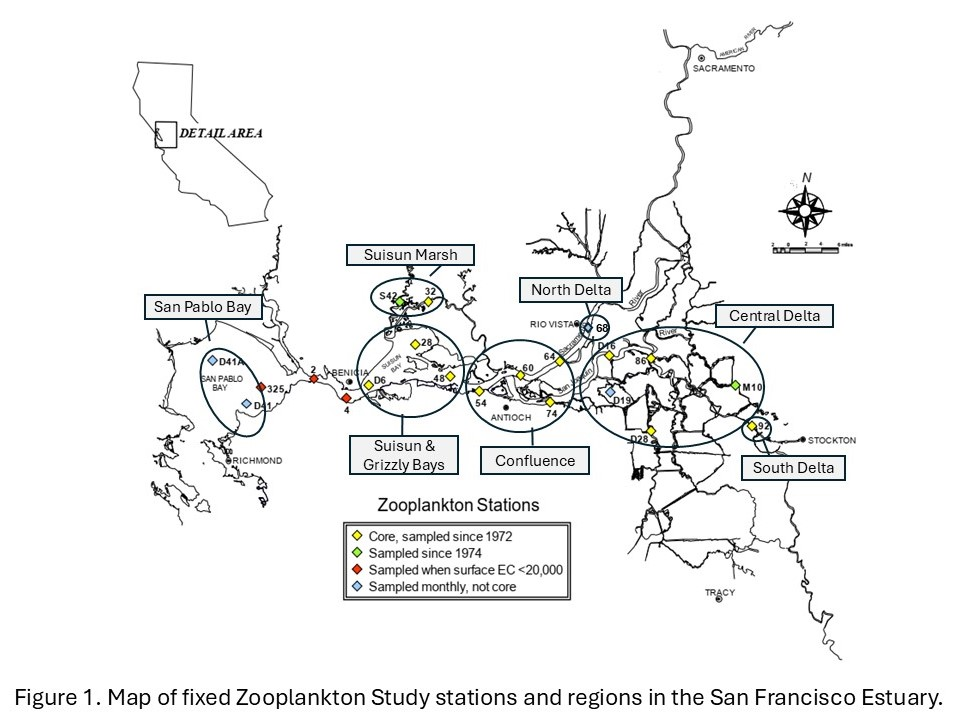
\includegraphics[width=0.85\linewidth,height=\textheight,keepaspectratio]{admin/figures-tables/zoop/zoop_station_map.jpg}

}

\caption{\label{fig-stations}}

\end{figure}%

\begin{center}
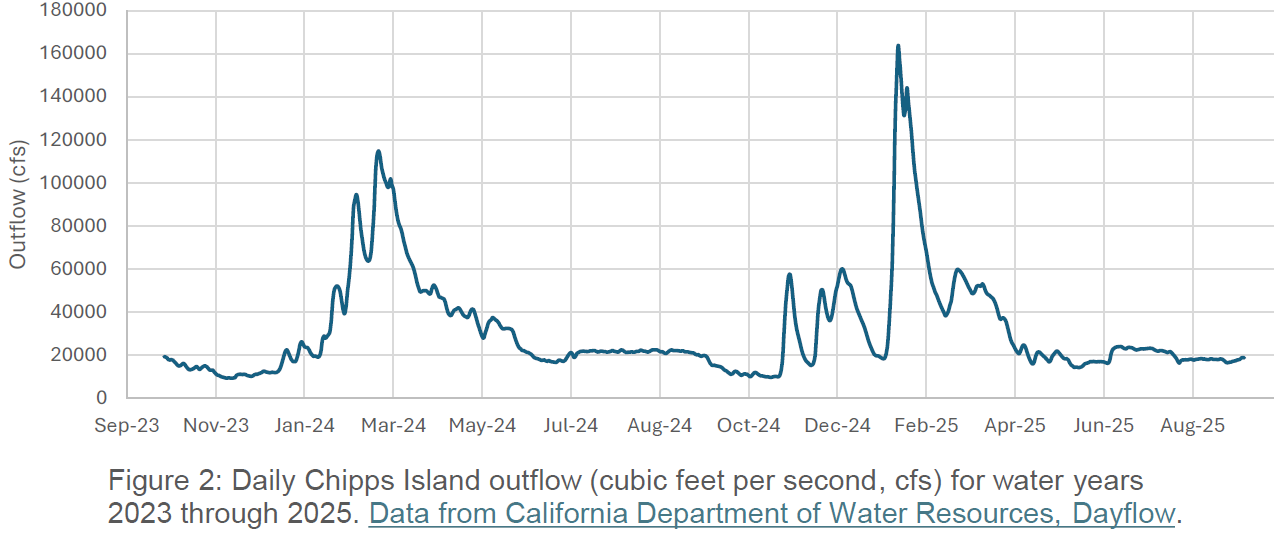
\includegraphics[width=0.8\linewidth,height=\textheight,keepaspectratio]{admin/figures-tables/zoop/zoop_fig2.png}
\end{center}

\begin{center}
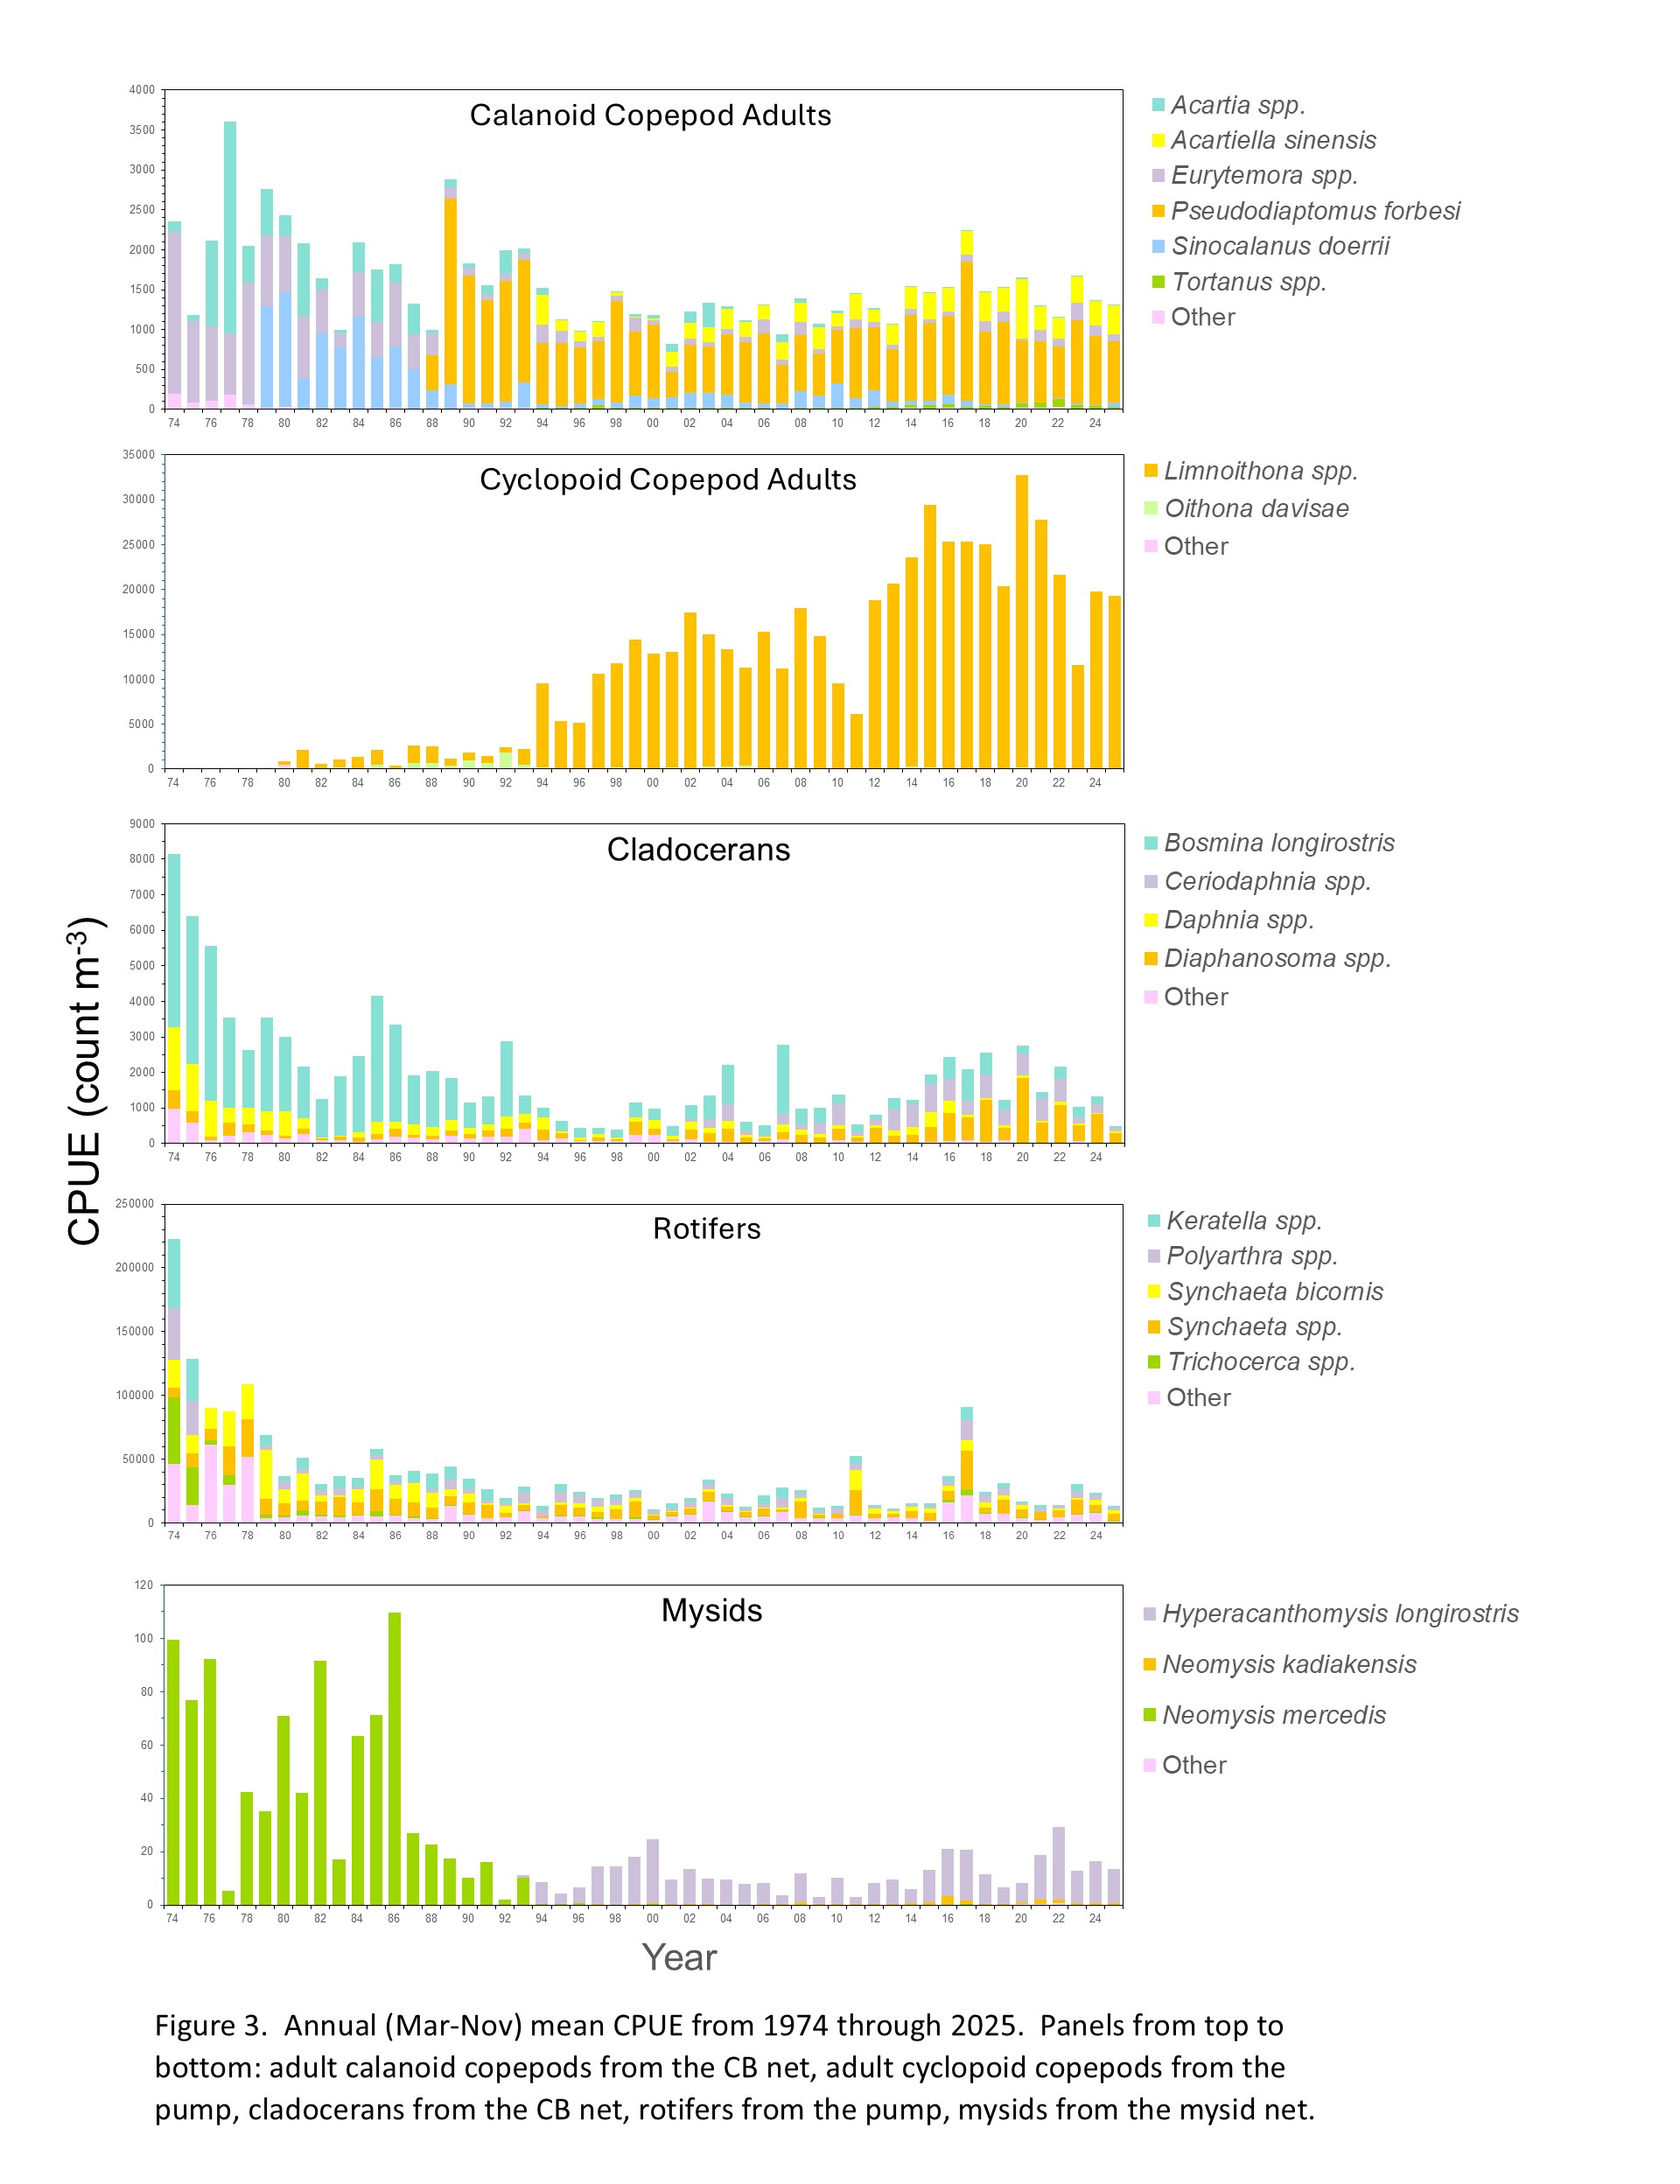
\includegraphics[width=0.85\linewidth,height=\textheight,keepaspectratio]{admin/figures-tables/zoop/zoop_fig3.jpg}
\end{center}

\begin{center}
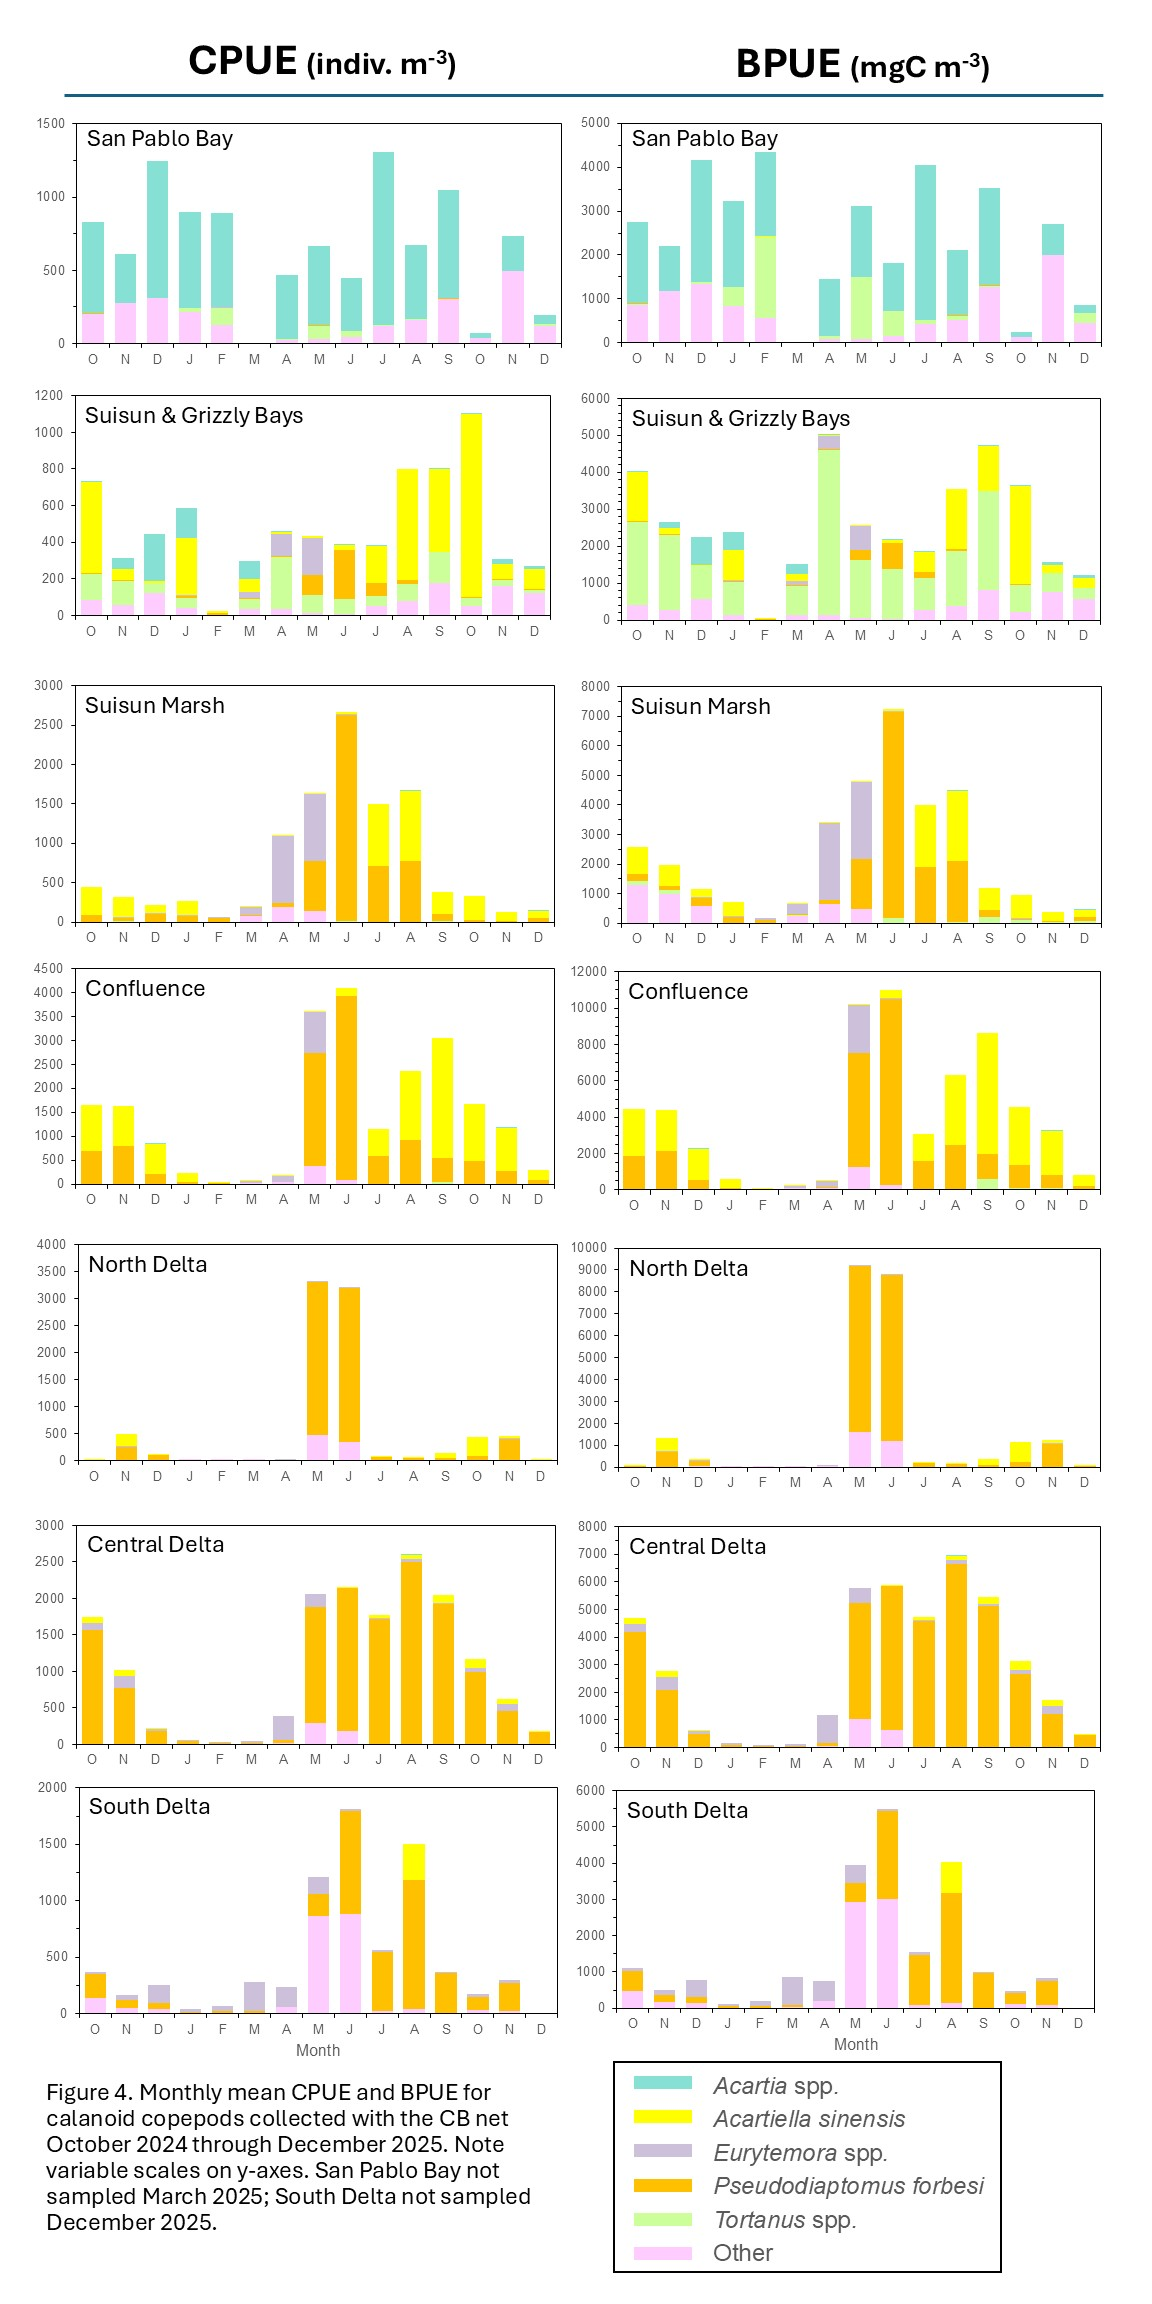
\includegraphics[width=0.85\linewidth,height=\textheight,keepaspectratio]{admin/figures-tables/zoop/zoop_fig4.jpg}
\end{center}

\begin{center}
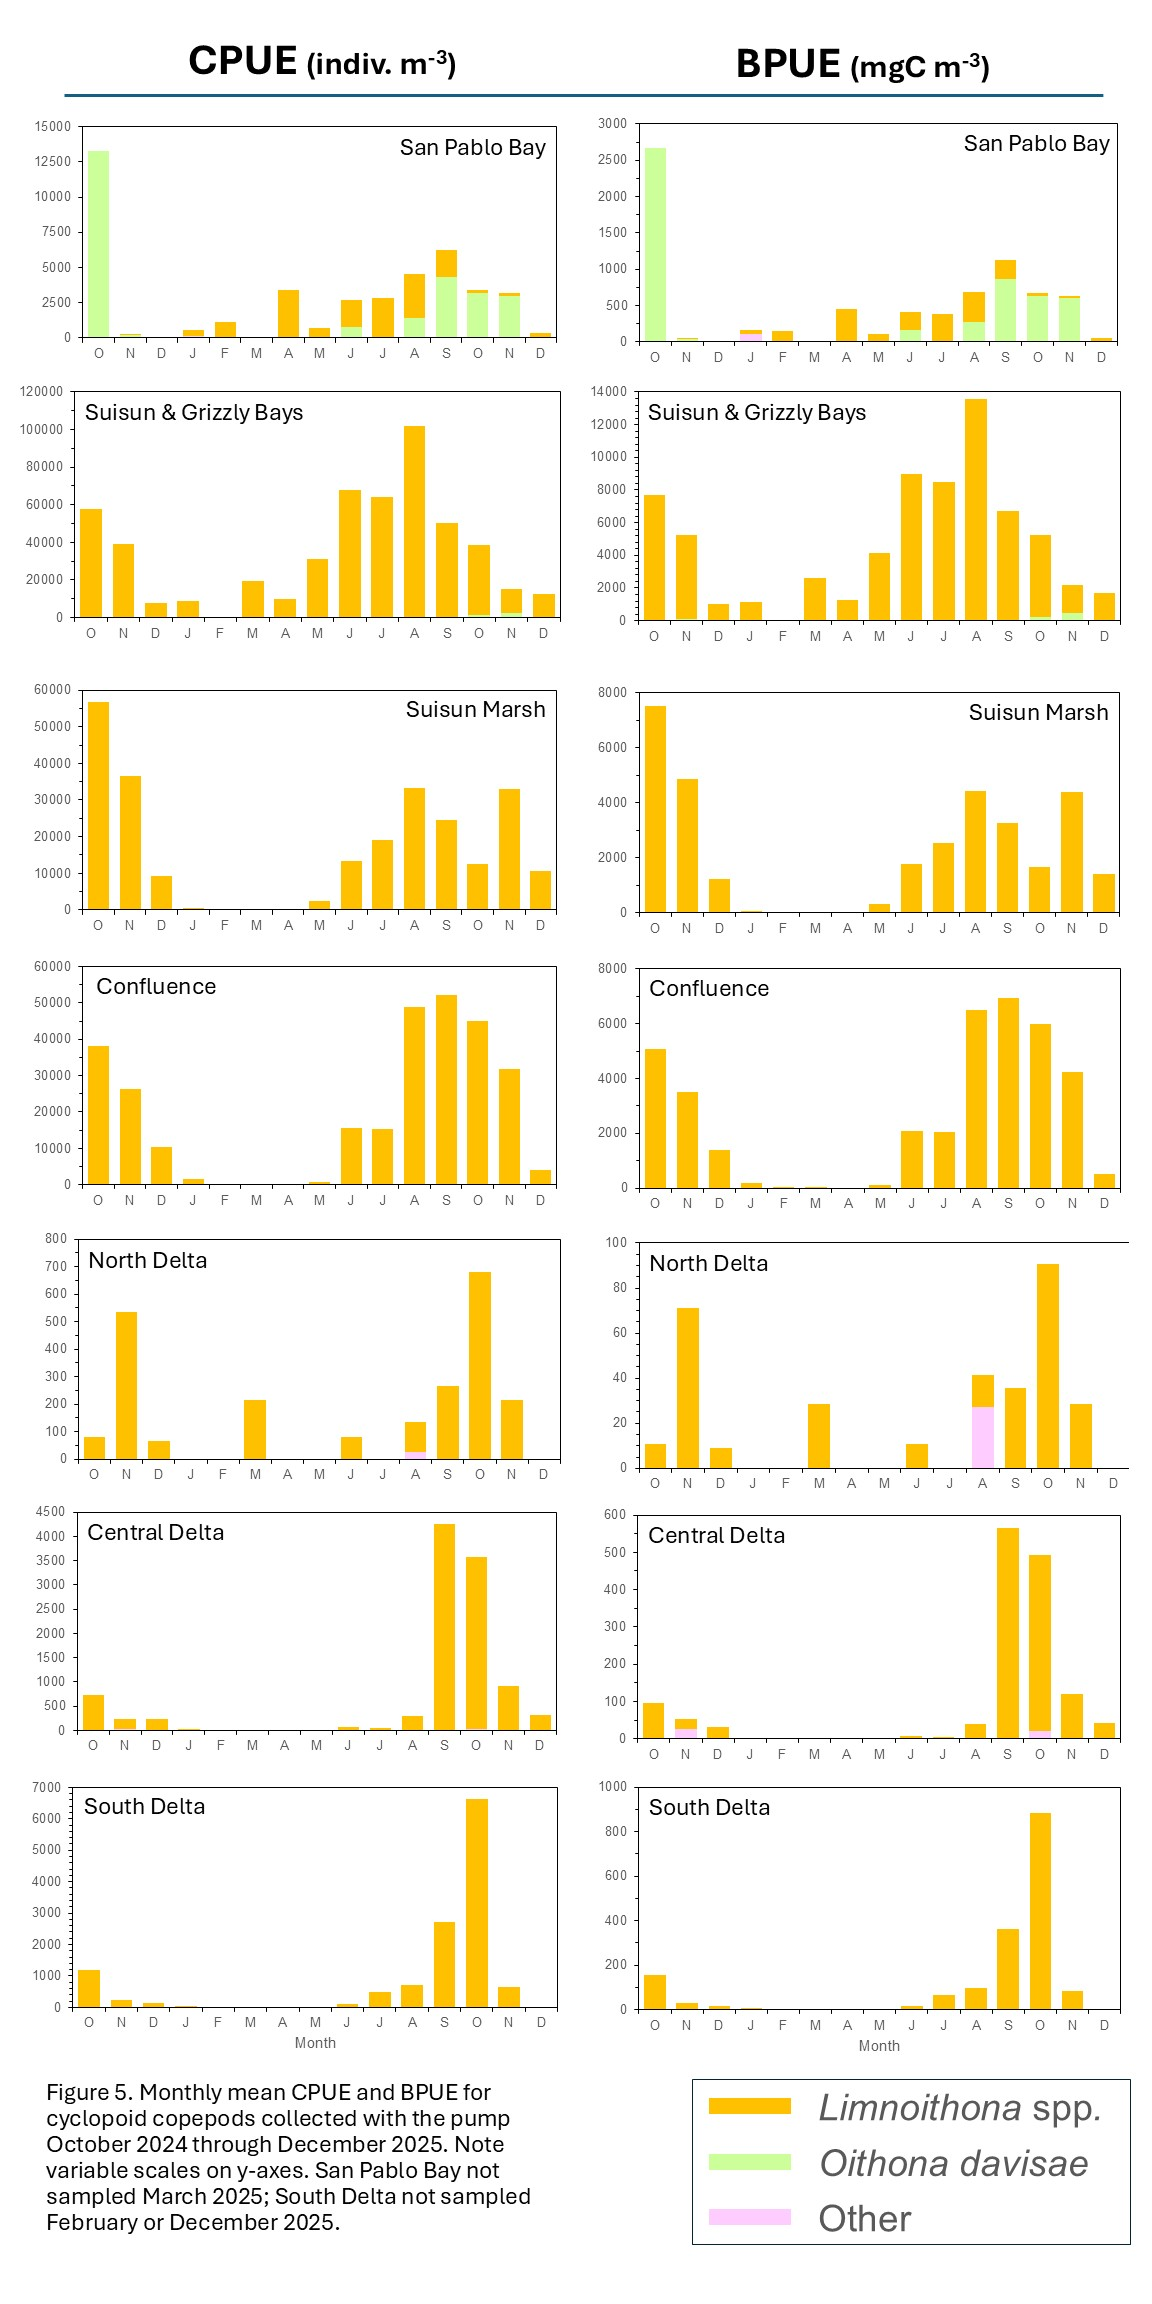
\includegraphics[width=0.85\linewidth,height=\textheight,keepaspectratio]{admin/figures-tables/zoop/zoop_fig5.jpg}
\end{center}

\begin{center}
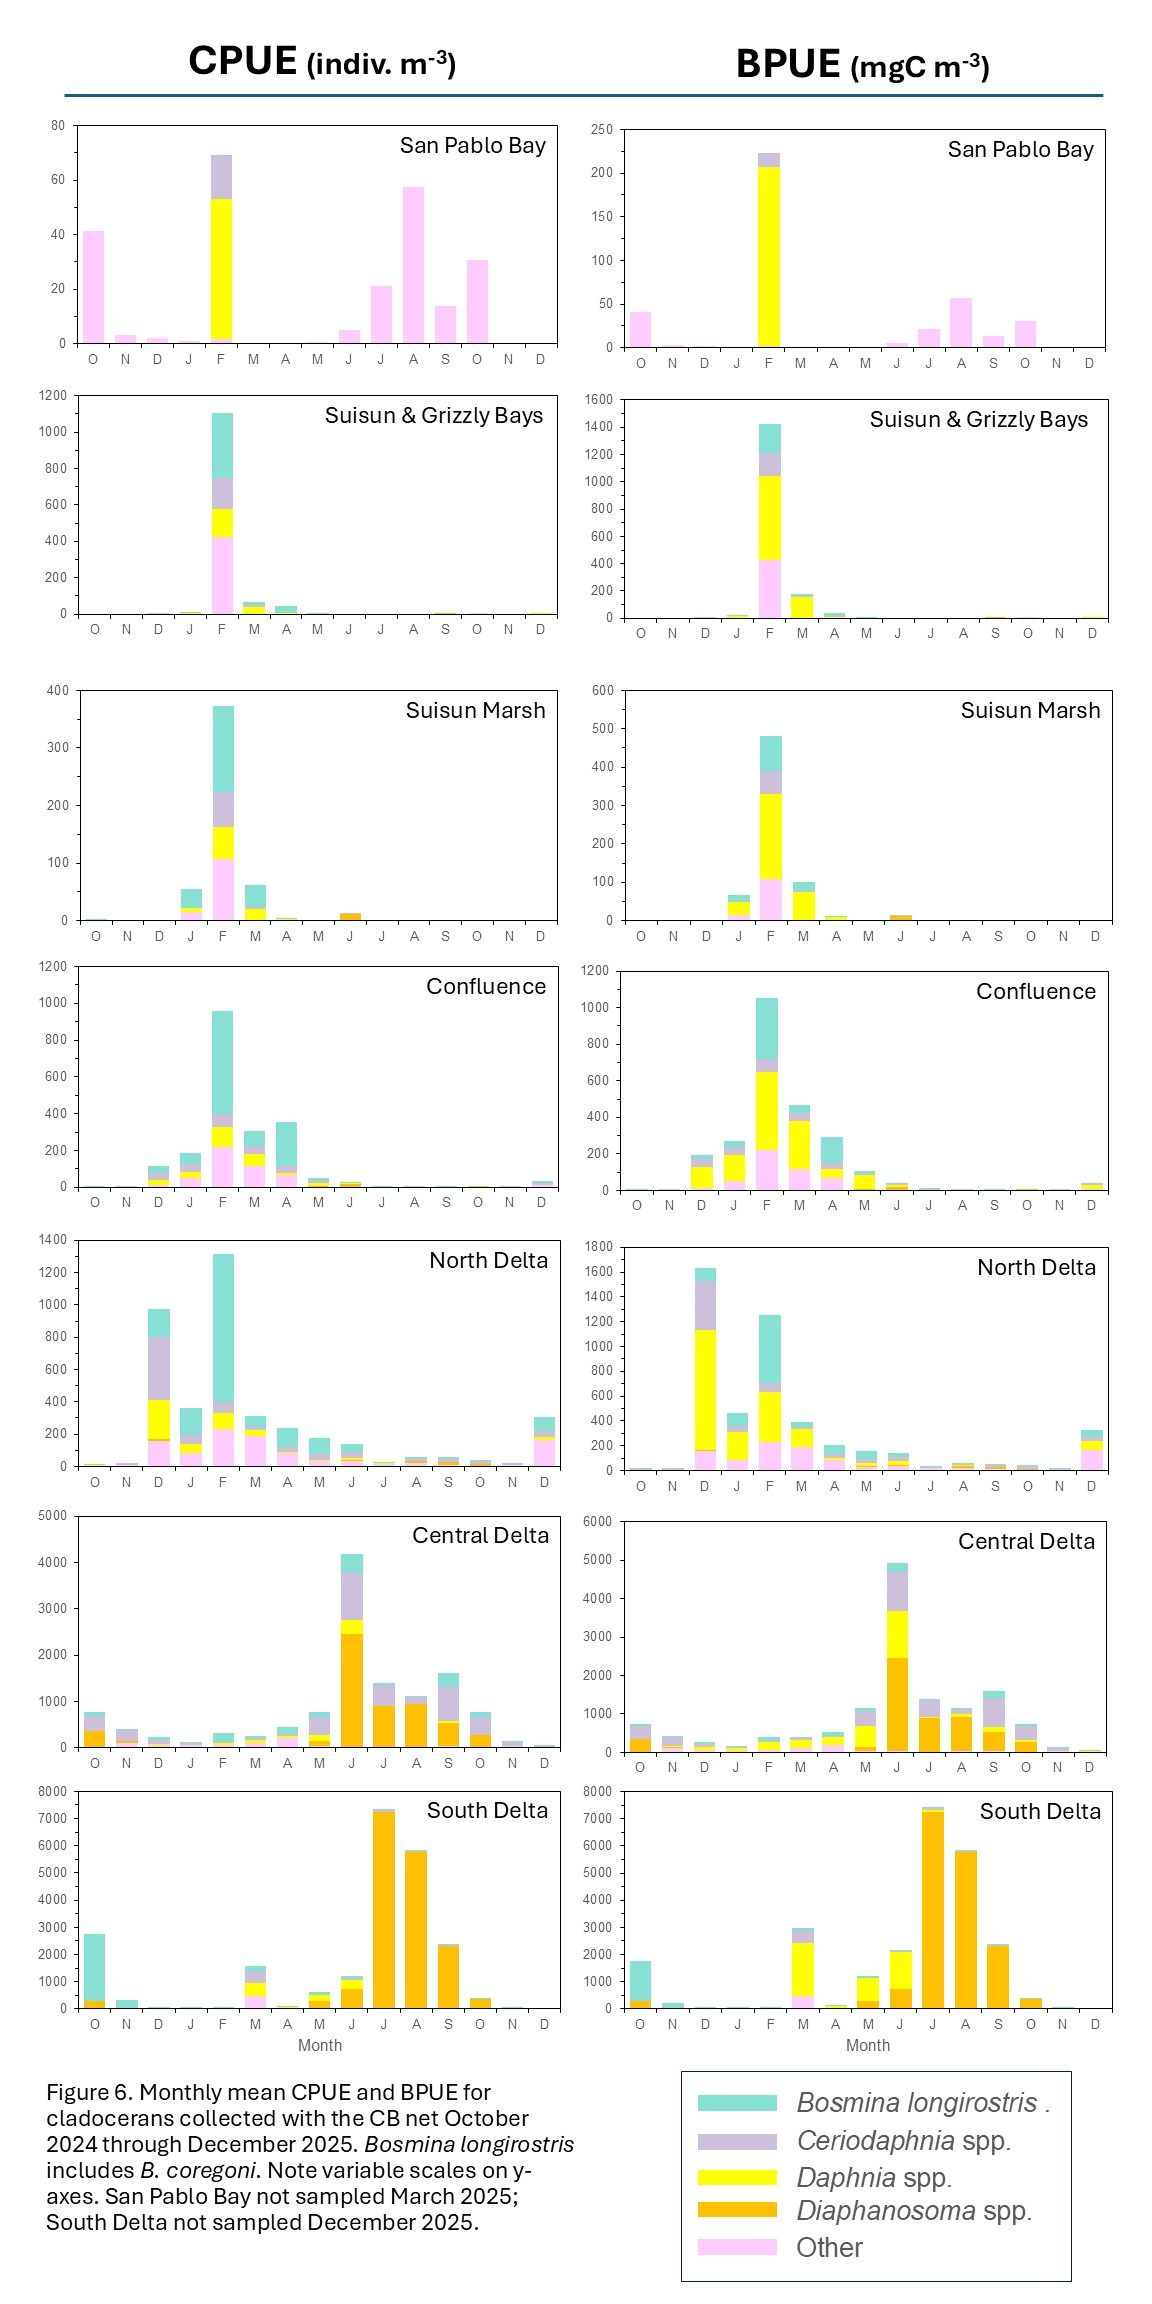
\includegraphics[width=0.85\linewidth,height=\textheight,keepaspectratio]{admin/figures-tables/zoop/zoop_fig6.jpg}
\end{center}

\begin{center}
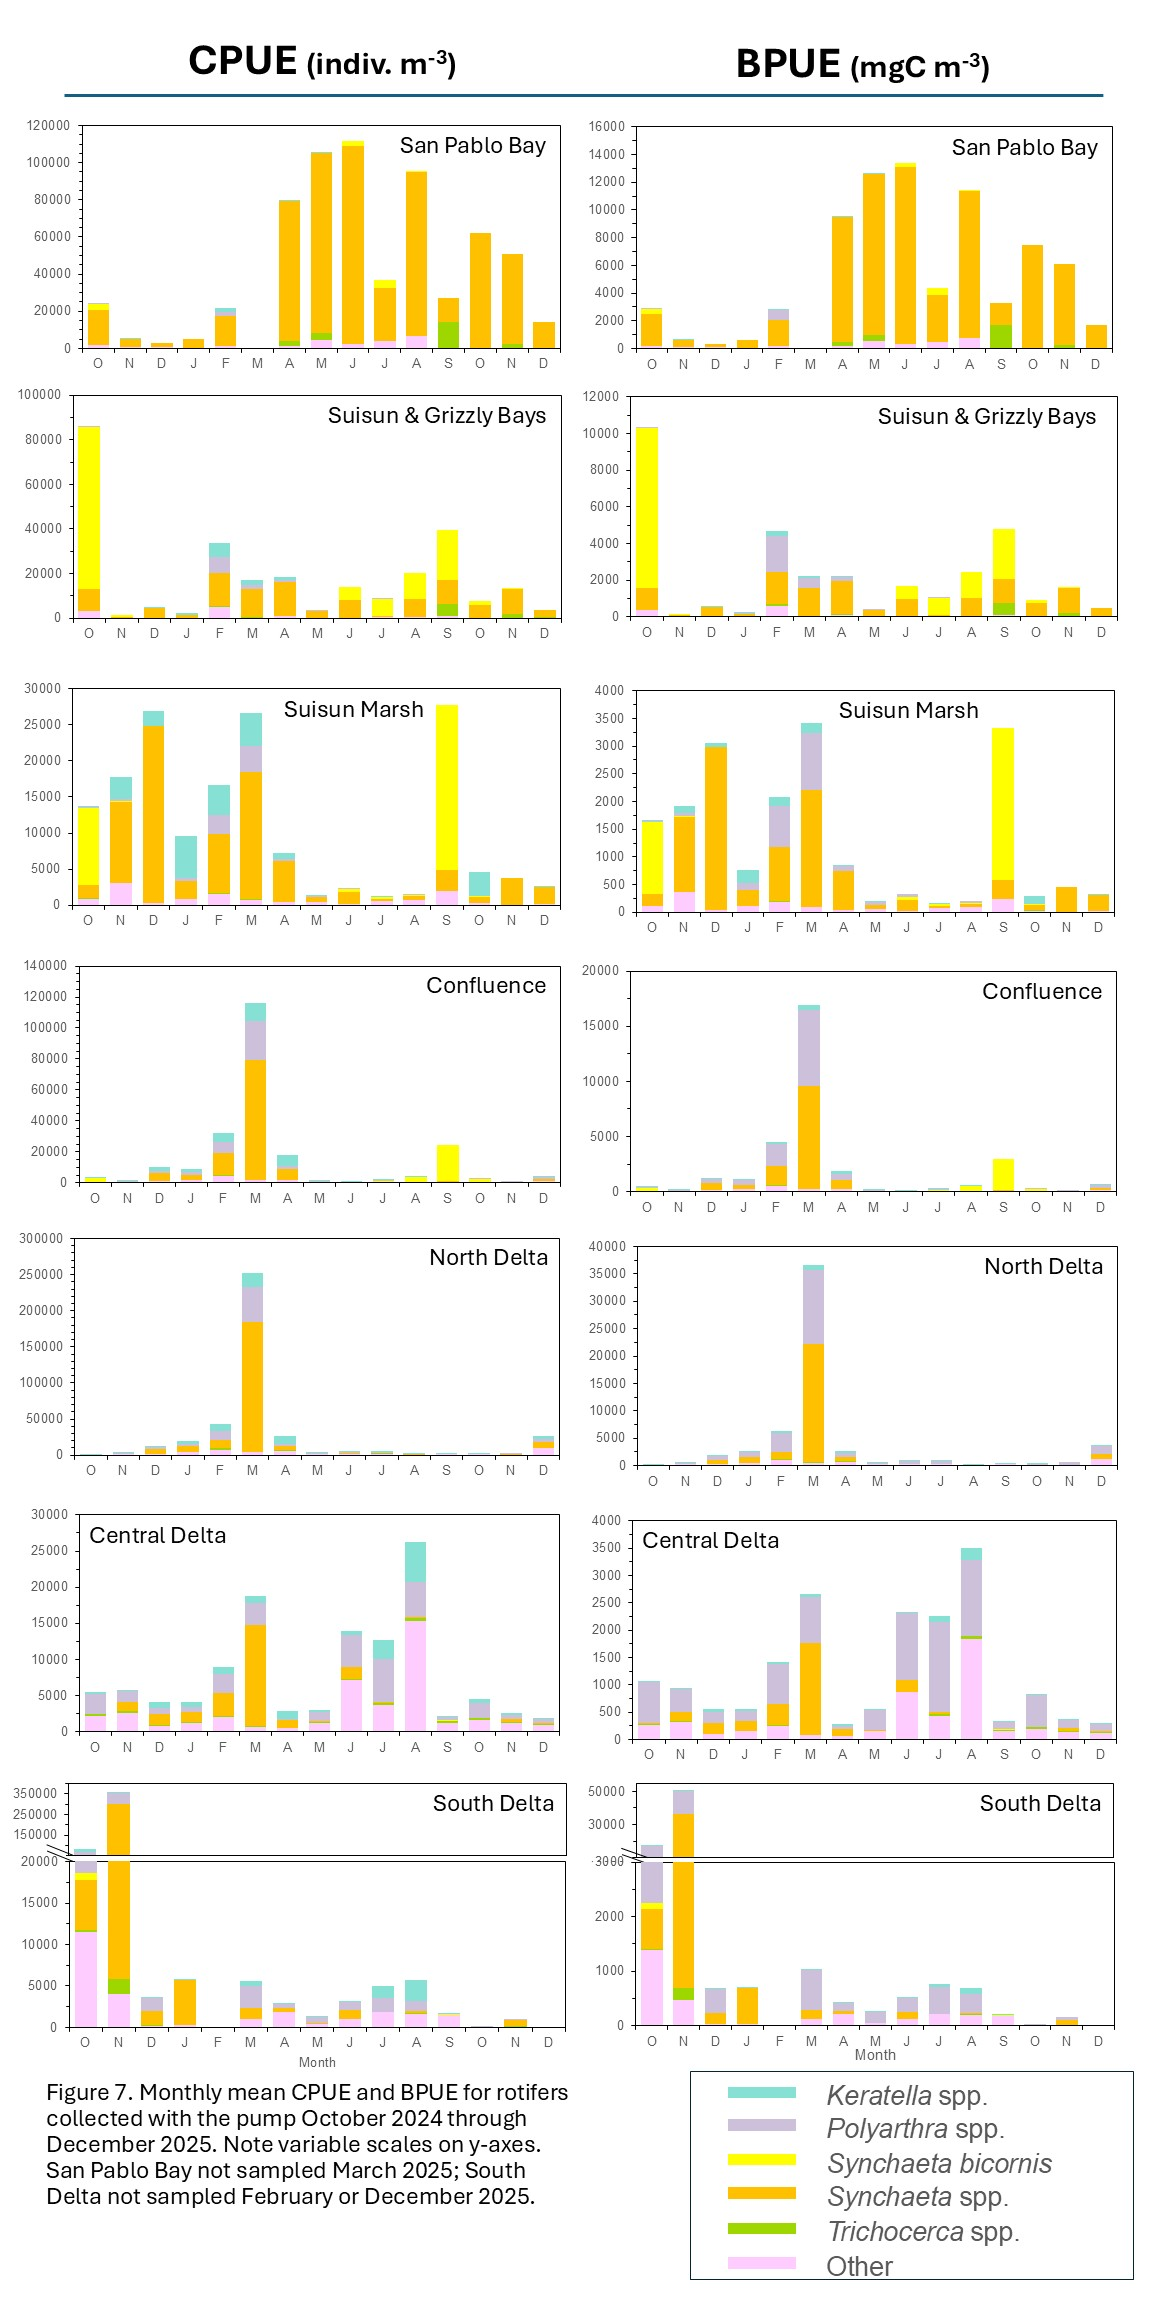
\includegraphics[width=0.85\linewidth,height=\textheight,keepaspectratio]{admin/figures-tables/zoop/zoop_fig7.jpg}
\end{center}

\begin{center}
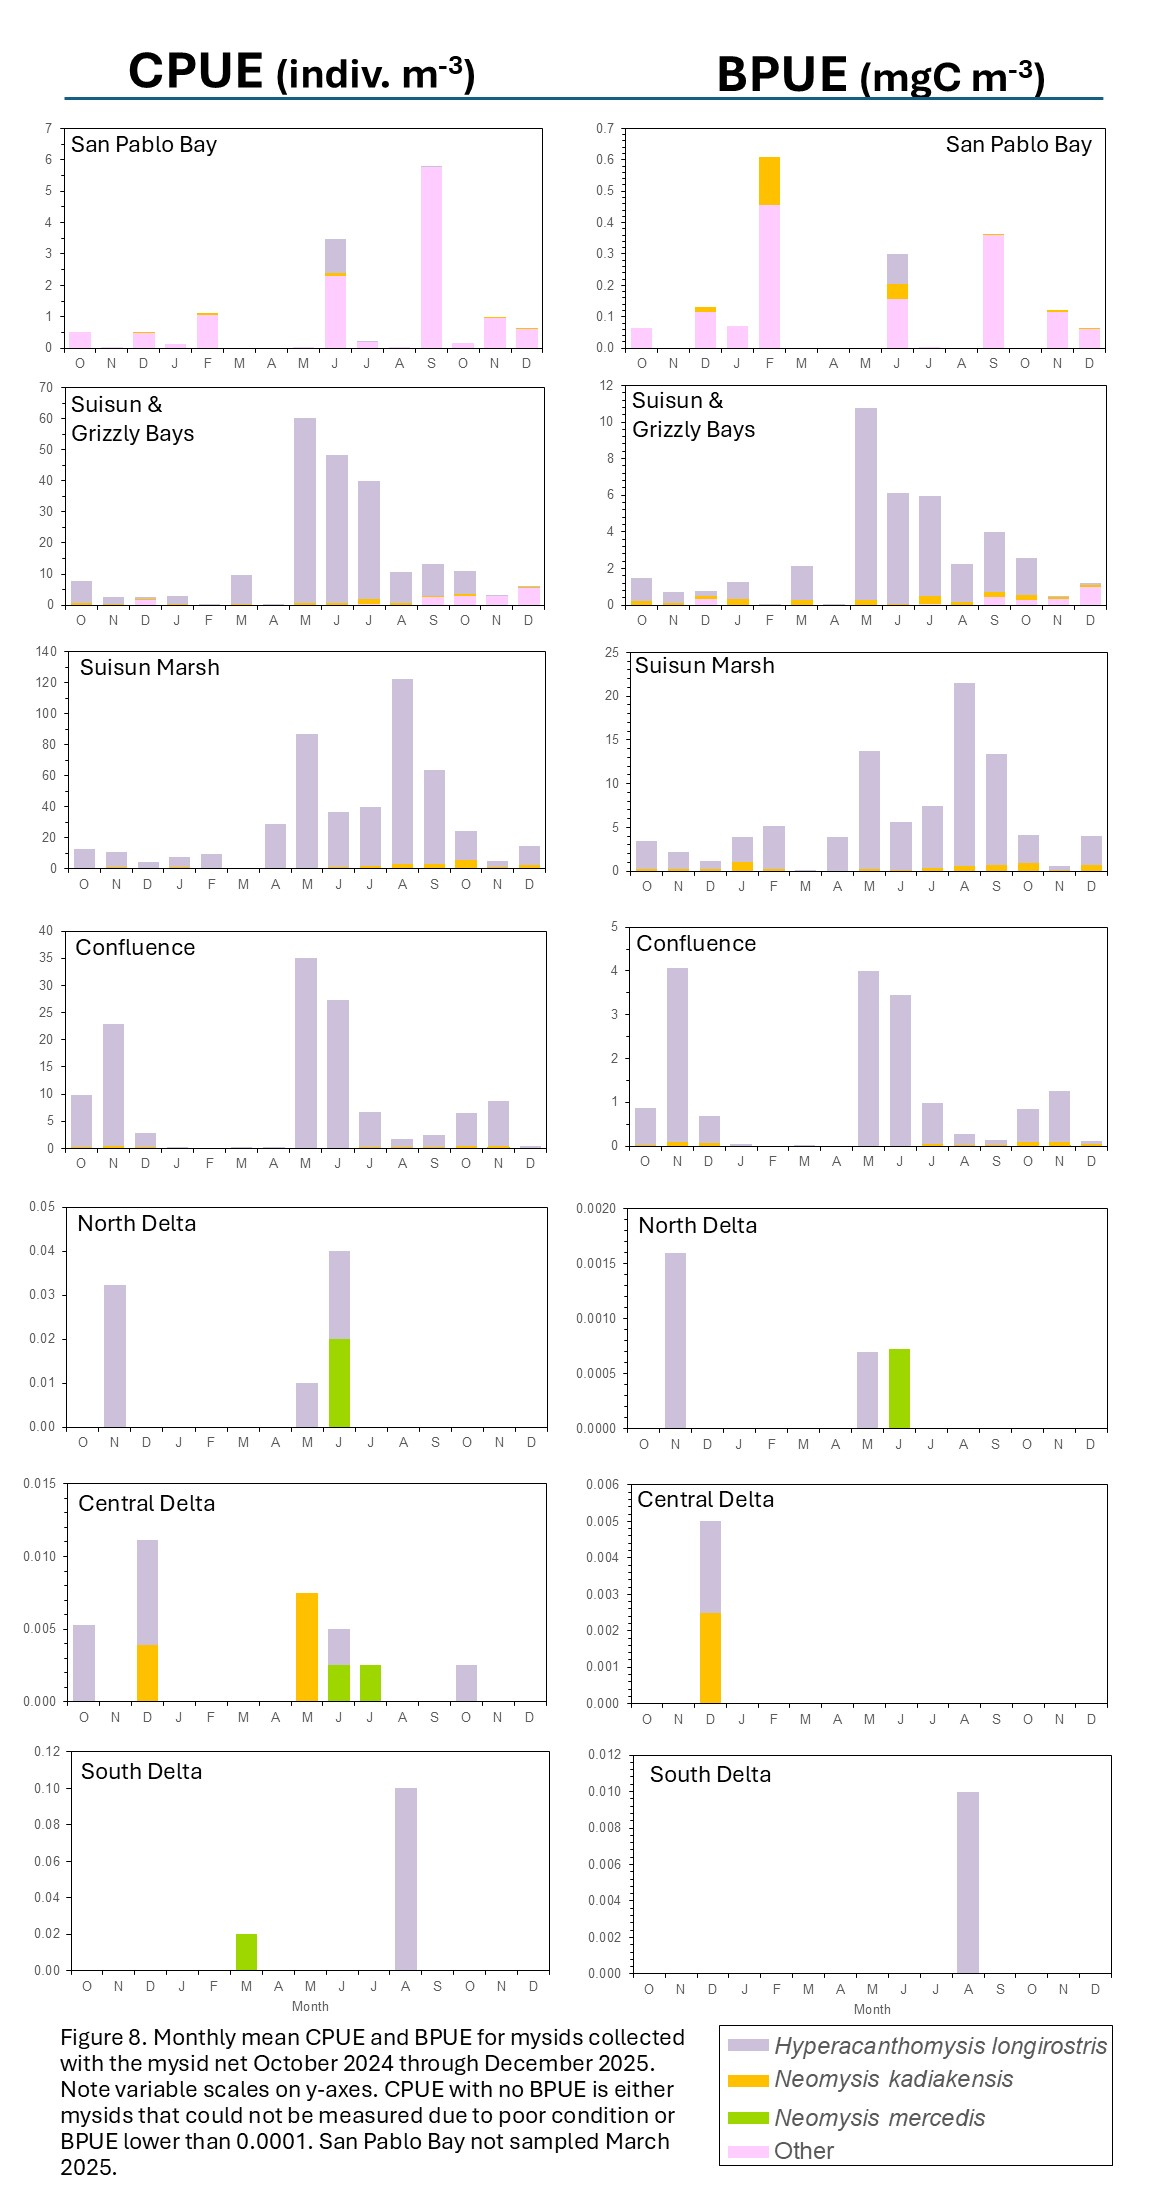
\includegraphics[width=0.85\linewidth,height=\textheight,keepaspectratio]{admin/figures-tables/zoop/zoop_fig8.jpg}
\end{center}




\end{document}
